%%%%%%%%%%%%%%%%%%%%%%% file typeinst.tex %%%%%%%%%%%%%%%%%%%%%%%%%%%%%%
%
% This is the LaTeX source for the instructions to authors using
% the LaTeX document class SVMultln with class option 'lnicst'
% for contributions to the Lecture Notes of the Institute for
% Computer Sciences, Social-Informatics and
% Telecommunications Engineering series.
% www.springer.com/series/XXXX       Springer Heidelberg 2007/08/05
%
% It may be used as a template for your own input - copy it
% to a new file with a new name and use it as the basis for
% your article. It contains a few tweaked sections to demonstrate
% features of the package, though.
%
% If you have not much experiences with Springer LaTeX support,
% you should better use the special demonstration file "lnicst.tex"
% included in the LaTeX package for LNICST as template.
%
%%%%%%%%%%%%%%%%%%%%%%%%%%%%%%%%%%%%%%%%%%%%%%%%%%%%%%%%%%%%%%%%%%%%%%%%

%\documentclass[lnicst,sechang,a4paper]{svmultln}
\documentclass{llncs} %this is for NSS
\bibliographystyle{splncs}
%\documentclass[runningheads,a4paper]{llncs} 



\usepackage{amssymb}
\setcounter{tocdepth}{3}
\usepackage{graphicx}


%\usepackage{amssymb}
%\setcounter{tocdepth}{3}
%\usepackage{graphicx}
%\usepackage{fancyhdr}
%\usepackage{lastpage}

\usepackage{url}

%\urldef{\mailsa}\path|{alfred.hofmann, ursula.barth, ingrid.haas, frank.holzwarth,|
%\urldef{\mailsb}\path|anna.kramer, leonie.kunz, christine.reiss, nicole.sator,|
%\urldef{\mailsc}\path|erika.siebert-cole, peter.strasser, lncs}@springer.com|    
%\newcommand{\keywords}[1]{\par\addvspace\baselineskip
%\noindent\keywordname\enspace\ignorespaces#1}


%added by the author himself
\usepackage[title]{appendix}
\usepackage{subfig}
\usepackage[]{algorithmicx}
\usepackage[]{algorithm}
\usepackage{algpseudocode}

\usepackage{color}
%\usepackage[numbers]{natbib}
\usepackage{calc}
\usepackage{siunitx}
\DeclareSIUnit\mt{\milli\tesla} %% A method for say short cut or new unit!
\sisetup{inter-unit-product = {-}}

\newcolumntype{P}[1]{>{\centering\arraybackslash}p{#1}}

\usepackage[T1]{fontenc}
\usepackage[ansinew]{inputenc}
\usepackage[english]{babel}
\usepackage{adjustbox}
\usepackage{amsmath,amsfonts,amssymb}
\usepackage{xparse}
\usepackage[section]{placeins} 
\usepackage[misc]{ifsym}
\usepackage{url}

 
\usepackage[many]{tcolorbox}
\usetikzlibrary{decorations.pathreplacing}

%added by kimmo
%\setlength\parskip{12pt}
%\setlength\parindent{0pt}
%\pagestyle{fancy}
%\fancyhf{} 
%\fancyfoot[C]{\thepage\ / \pageref{LastPage}}
%\renewcommand{\headrulewidth}{0pt}



\begin{document}



\mainmatter  % start of an individual contribution

% first the title is needed
\title{On De-synchronization of User Pseudonyms in Mobile Network}
%Concealing IMSI in 5G Network Using Identity Based Cryptography

% a short form should be given in case it is too long for the running head
%\titlerunning{Concealing IMSI Using Identity Based Encryption} 


% the name(s) of the author(s) follow(s) next
%
% NB: Chinese authors should write their first names(s) in front of
% their surnames. This ensures that the names appear correctly inlso
% the running heads and the author index.
%
\author{Mohsin Khan$^\text{1(\Letter)}$%
%%\thanks{Please note that the LNICST Editorial assumes that all authors have used
%%the western naming convention, with given names preceding surnames. This determines
%%the structure of the names in the running heads and the author index.}%
\and Kimmo J\"arvinen$^\text{1}$
\and Philip Ginzboorg$^\text{2,3}$
\and Valtteri Niemi$^\text{1}$
}  %

%\authorrunning{Mohsin Khan \and Valtteri Niemi}

% (feature abused for this document to repeat the title also on left hand pages)

% the affiliations are given next
\institute{$^\text{1}$University of Helsinki, Helsinki, Finland\\
\{\email{mohsin.khan, kimmo.u.jarvinen, valtteri.niemi}\}\email{@helsinki.fi}\\
$^\text{2}$ Huawei Technologies, Helsinki, Finland\\
$^\text{3}$ Aalto University, Espoo, Finland\\
\email{philip.ginzboorg@huawei.com}
%P.O. Box 68 (Gustaf H\"allstr\"omin katu 2b)\\
%FI-00014 University of Helsinki\\
%Finland\\
%\url{https://www.cs.helsinki.fi/en}
}

%relationship stu
%
% NB: a more complex sample for affiliations and the mapping to the
% corresponding authors can be found in the file "lnicst.dem",
% that is contained in the LNICST LaTeX support package.
%

%%%\toctitle{Lecture Notes in Computer Science}
%%%\tocauthor{Authors' Instructions}
\maketitle


\begin{abstract}
This paper is in the area of pseudonym-based enhancements of user identity privacy in mobile networks. Khan and Mitchell (2017) have found that in recently published pseudonym-based schemes an attacker can desynchronize the pseudonyms' state in the user equipment and in its home network.  In this paper, we first show that exploiting this vulnerability a botnet of mobile devices can kick out of service a large portion of mobile network users.  We characterize this novel  DDoS attack analytically and confirm our analysis using a simulation. Second, we explain how to modify the pseudonym-based schemes in order to mitigate the DDoS attack. The proposed solution is simpler than that in Khan and Mitchell (2017). We also discuss aspects of pseudonym usage in mobile network from charging and regulatory point of view.
\keywords{3GPP $\cdot$ IMSI catchers $\cdot$ Pseudonym $\cdot$ Identity $\cdot$ Privacy}
\end{abstract}


\section{Introduction} \label{intro}
International mobile subscriber identity (IMSI) catchers are threats to the identity privacy of mobile users. Passive IMSI catchers are devices that observe the wireless traffic and store all the IMSIs observed. Active IMSI catchers are malicious devices that can trick a user equipment (UE) to reveal its IMSI. Protection against passive IMSI catchers has been in the cellular networks since the second generation (GSM). However, active IMSI catchers have persisted in all the cellular networks, namely, GSM, UMTS and LTE \cite{mobicom95,imsi_catcher_report_bochum,Ginzboorg_Niemi_2016,washingtonpost2014,pets2017,pki_umts_imsi_catcher}. 

%\subsubsection{IMSI Catching}
%The network a UE has a subscription with is called the home network (HN). The network a UE visits and gets services from is called serving network (SN). In an ideal situation, a UE has to identify and authenticate itself to an SN before receiving any services from it. In cellular networks the encryption key in a UE is generated using the pre-shared symmetric key during authentication \cite{TS33401}. So, before authentication, neither a UE nor the SN/HN knows the key to use for encryption or decryption.  Consequently, the identity of the UE has to be sent in plaintext to the SN. This enables an active IMSI catcher to play its trick.

An active IMSI catcher impersonates a legitimate serving network (SN) and asks for the identity of all the UEs in the range of the IMSI catcher. The UEs have no way to differentiate an IMSI catcher from a legitimate SN, hence reveal their IMSIs as if they were revealing to a legitimate SN. 

%An IMSI catcher can exploit the knowledge of caught IMSIs to monitor and track the physical location of a mobile user \cite{tracking_bins,goldman2007mobile}. Please note that the term "IMSI catcher" is also used in a wider meaning, referring to extended attacks, including man-in-the-middle type of attacks or just spamming \cite{catch_me_if_you_can,chinese_spam}. In this paper we limit our discussion only to prevent the IMSI catchers from catching the IMSIs (identities) of the users.

%Different kind of solutions to defeat IMSI catchers have been proposed over the years. In addition to protect privacy, a desirable property of the solution is backward compatibility, i.e., it should protect the identity privacy even in the presence of a legacy SN. This is because, if the solution to defeat IMSI catchers works only in the latest generation of cellular network (e.g., 5G), then an attacker may be able to mount a downgrade attack. 

%\subsubsection{Pseudonym Based Solutions}
A potentially simple and backward compatible solution approach is to use frequently-changing temporary identities for mobile users \cite{CCS15,SSR15,Ginzboorg_Niemi_2016,Norrman_Naslund_Dubrova_2016,yemen2017}. The idea is, even if an IMSI catcher plays its trick, only the temporary identity of a user would be revealed. So, the IMSI catcher would not be able to associate the temporary identity with any user who is previously known. The temporary identities are called pseudonyms, hence the solutions use this approach are called pseudonym based solutions. 

Borek, Verdult, and Ruiter \cite{CCS15} and Khan and Mitchell \cite{SSR15}, described solutions based on pseudonyms that have the same format as IMSIs. From now on we will refer these two schemes as BVR and KM15 schemes. These solutions are prone to the loss of synchronization between the pseudonyms in the UE and the home network (HN) of the user. In the worst loss of synchronization case, there is not even one pseudonym left in the UE that the HN accepts. Hence all the identification and authentication attempt would fail thereafter and the UE would go out of the service. There is a vulnerability in these solutions that can be exploited by an attacker to cause the loss of pseudonym synchronization. The attacker can be a malicious UE or a malicious SN.

Khan and Mitchel \cite{wisec17} identified the loss of synchronization problem caused by a malicious UE and proposed a solution. In the rest of the paper we will refer to this solution as KM17 scheme. Careful investigation into this scheme shows that a UE has to use one pseudonym at least twice before it can get a new pseudonym from the network. The authors also argue that their solution may be vulnerable to a pseudonym de-synchronization attack by a malicious SN. To address the issue of malicious SNs, they introduce an identity recovery procedure. But this procedure adds complexity: the number of temporary identities per user increases from two to six. Moreover, as we will explain, the recovery mechanism itself can be exploited by an IMSI catcher to track the mobile user.

%\begin{figure}[!tbp]
%  \centering
%  \begin{minipage}[b]{0.44\textwidth}
%    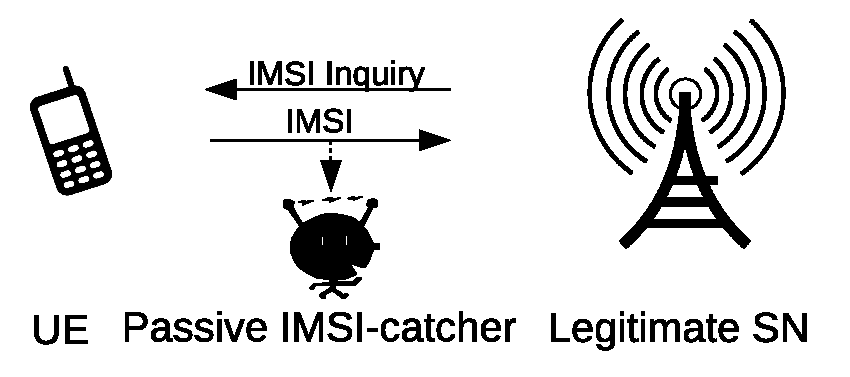
\includegraphics[width=\textwidth]{Passive_IMSI-Catcher.eps}
%    \caption{Legitimate SN}
%  \end{minipage}
%  \hfill
%  \begin{minipage}[b]{0.50\textwidth}
%    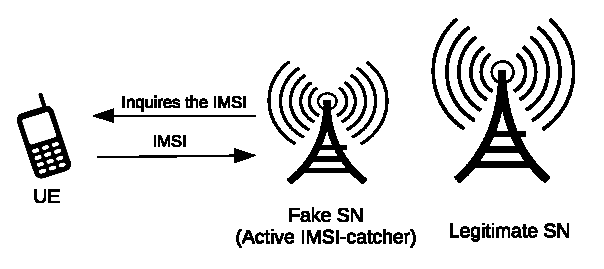
\includegraphics[width=\textwidth]{Active-IMSI-Cactcher.eps}
%    \caption{IMSI-catcher}
%  \end{minipage}
%  \caption{IMSI-catcher}
%  \label{fig:IMSI-catching}
%\end{figure}

\textbf{Our Contribution:}
We propose a pseudonym based solution that builds on top of those in BVR, KM15 and KM17 schemes. The following contributions are made:
\begin{enumerate}
\item Identify a DDoS attack against an entire HN when the BVR scheme is used.
\item Design a solution that corrects the weaknesses of the KM17 scheme and is simpler than that scheme.
\item Outline some practical concerns of using pseudonyms from billing and regulatory point of view.
\end{enumerate}




\section{Preliminaries}
Conceptually, a cellular network can be divided into UE; the HN -- where the mobile user has a subscription; and the SN -- that is the network to which mobile device connects.  The SN and HN are the same when the user is not roaming. An SN or HN consist of many entities. In this paper we will not discuss those fine details. However, we need to know some detail about a UE. A UE consists of two entities. A mobile equipment (ME) and a subscriber identity module (SIM). The SIM is known as universal subscriber module (USIM) in UMTS. SIM or USIM, they are smart cards which are portable across different MEs. In LTE, the USIM is an application in the universal integrated circuit card (UICC). In this paper, for the sake of simplicity we will refer all of them as SIM.


A user is identified by IMSI. IMSI is a string of $15$ decimal digits. An IMSI is a concatenation of mobile country code (MCC), mobile network code (MNC) and mobile subscription identification number (MSIN). MCC is a string of $3$ decimal digits. MNC is of $2$ to $3$ decimal digits and MSIN is of $9$ to $10$ decimal digits. Pseudonyms discussed in this paper are IMSI looking strings. In this paper we limit our discussion to only one HN. Consequently all the IMSIs or pseudonyms we discuss have the same MCC and MNC. When we talk about IMSI space or pseudonym space, we actually mean the MSIN space. We denote the size of this space by $\mathcal{M}$. The value of $\mathcal{M}$ can be either $10^9$ or $10^{10}$. We will also use $n$ to denote the total number of users subscribed with an HN.

In the cellular networks, the security is built on a pre-shared master key $\mathcal{K}$ between a user and its HN. The key $\mathcal{K}$ is stored in the SIM along with the IMSI. The HN maintains a map from IMSI to key $\mathcal{K}$ for all the users. The authentication mechanism used by an SN to authenticate a user is based on challenge and response. The key $\mathcal{K}$ is only known by the HN, hence the HN delegates the SN by sending the challenge and expected response. %We will soon describe the authentication mechanism in UMTS and LTE briefly. But before that, we mention the use of temporary mobile subscription identity (TMSI) and globally unique temporary UE identity (GUTI).
Pseudonyms are assigned to a user during the authentication. This requires to make certain changes in the authentication protocol. In UMTS and LTE, the authentication protocols are called UMTS AKA and LTE AKA respectively. Before we discuss the pseudonym based solutions, we present UMTS AKA  and LTE AKA briefly.

%Once a user is authenticated by the SN, the user is given a temporary identity by the SN with confidentiality protection. The temporary identity is used by the SN and UE thereafter to identify the user so that anyone listening to the radio traffic can not identify the user. The temporary identity is known as TMSI in GSM and UMTS networks, and as GUTI in LTE network. The use of TMSI and GUTI can not defeat the IMSI catchers because the SN can still make an IMSI inquiry to a UE. Hence an IMSI catcher impersonating a legitimate SN can also make an IMSI inquiry. 

%TMSI or GUTI is assigned to a UE by the SN. They are assigned with confidentiality protection after the authentication is successful and necessary security context has been set up. However, pseudonyms are assigned by the HN and no security context is set up between a UE and an HN after authentication. Hence, the idea is to assign the pseudonym to a user during the authentication. This requires to make certain changes in the authentication protocol. In UMTS and LTE, the authentication protocols are called UMTS AKA and LTE AKA respectively. LTE AKA has a very little difference compared with UMTS AKA. Before we discuss the pseudonym based solutions, we present UMTS AKA  and LTE AKA briefly.

\subsection{UMTS/LTE AKA}
We discuss UMTS and LTE AKA only very briefly so that we can make a smooth transition to the discussion of pseudonym based solution. Details of UMTS AKA can be found in clause 6.3 of 3GPP TS 33.102 \cite{TS33102} and LTE AKA can be found in clause 6 of 3GPP TS 33.401 \cite{TS33401}. 

The UE identifies itself using the IMSI to the SN while sending an attach request or responding to an IMSI inquiry. Upon receiving the IMSI, an SN sends an authentication vector (AV) request to the HN for the IMSI. The HN finds the pre-shared key $\mathcal{K}$, randomly generate a challenge ($RAND$) and compute the expected response ($XRES$), two keys $CK$ and $IK$ as function of $\mathcal{K}$ and $RAND$. The HN also computes a string called $AUTN$ for the purpose of some cryptographic protections of the authentication protocol. HN forwards $RAND,AUTN,XRES, CK,IK$ to the SN. SN forwards the $RAND,AUTN$ to the UE. The UE verifies the $AUTN$, computes $SRES,CK,IK$ using the $RAND$ and key $\mathcal{K}$ and forwards $SRES$ to the SN. If $SRES$ and $XRES$ are the same strings, then the authentication is successful. The keys $CK$ and $IK$ are used for confidentiality and integrity protection thereafter. See Figure \ref{fig:UMTS_LTE_AKA}.

\begin{figure}[]
  \centering
    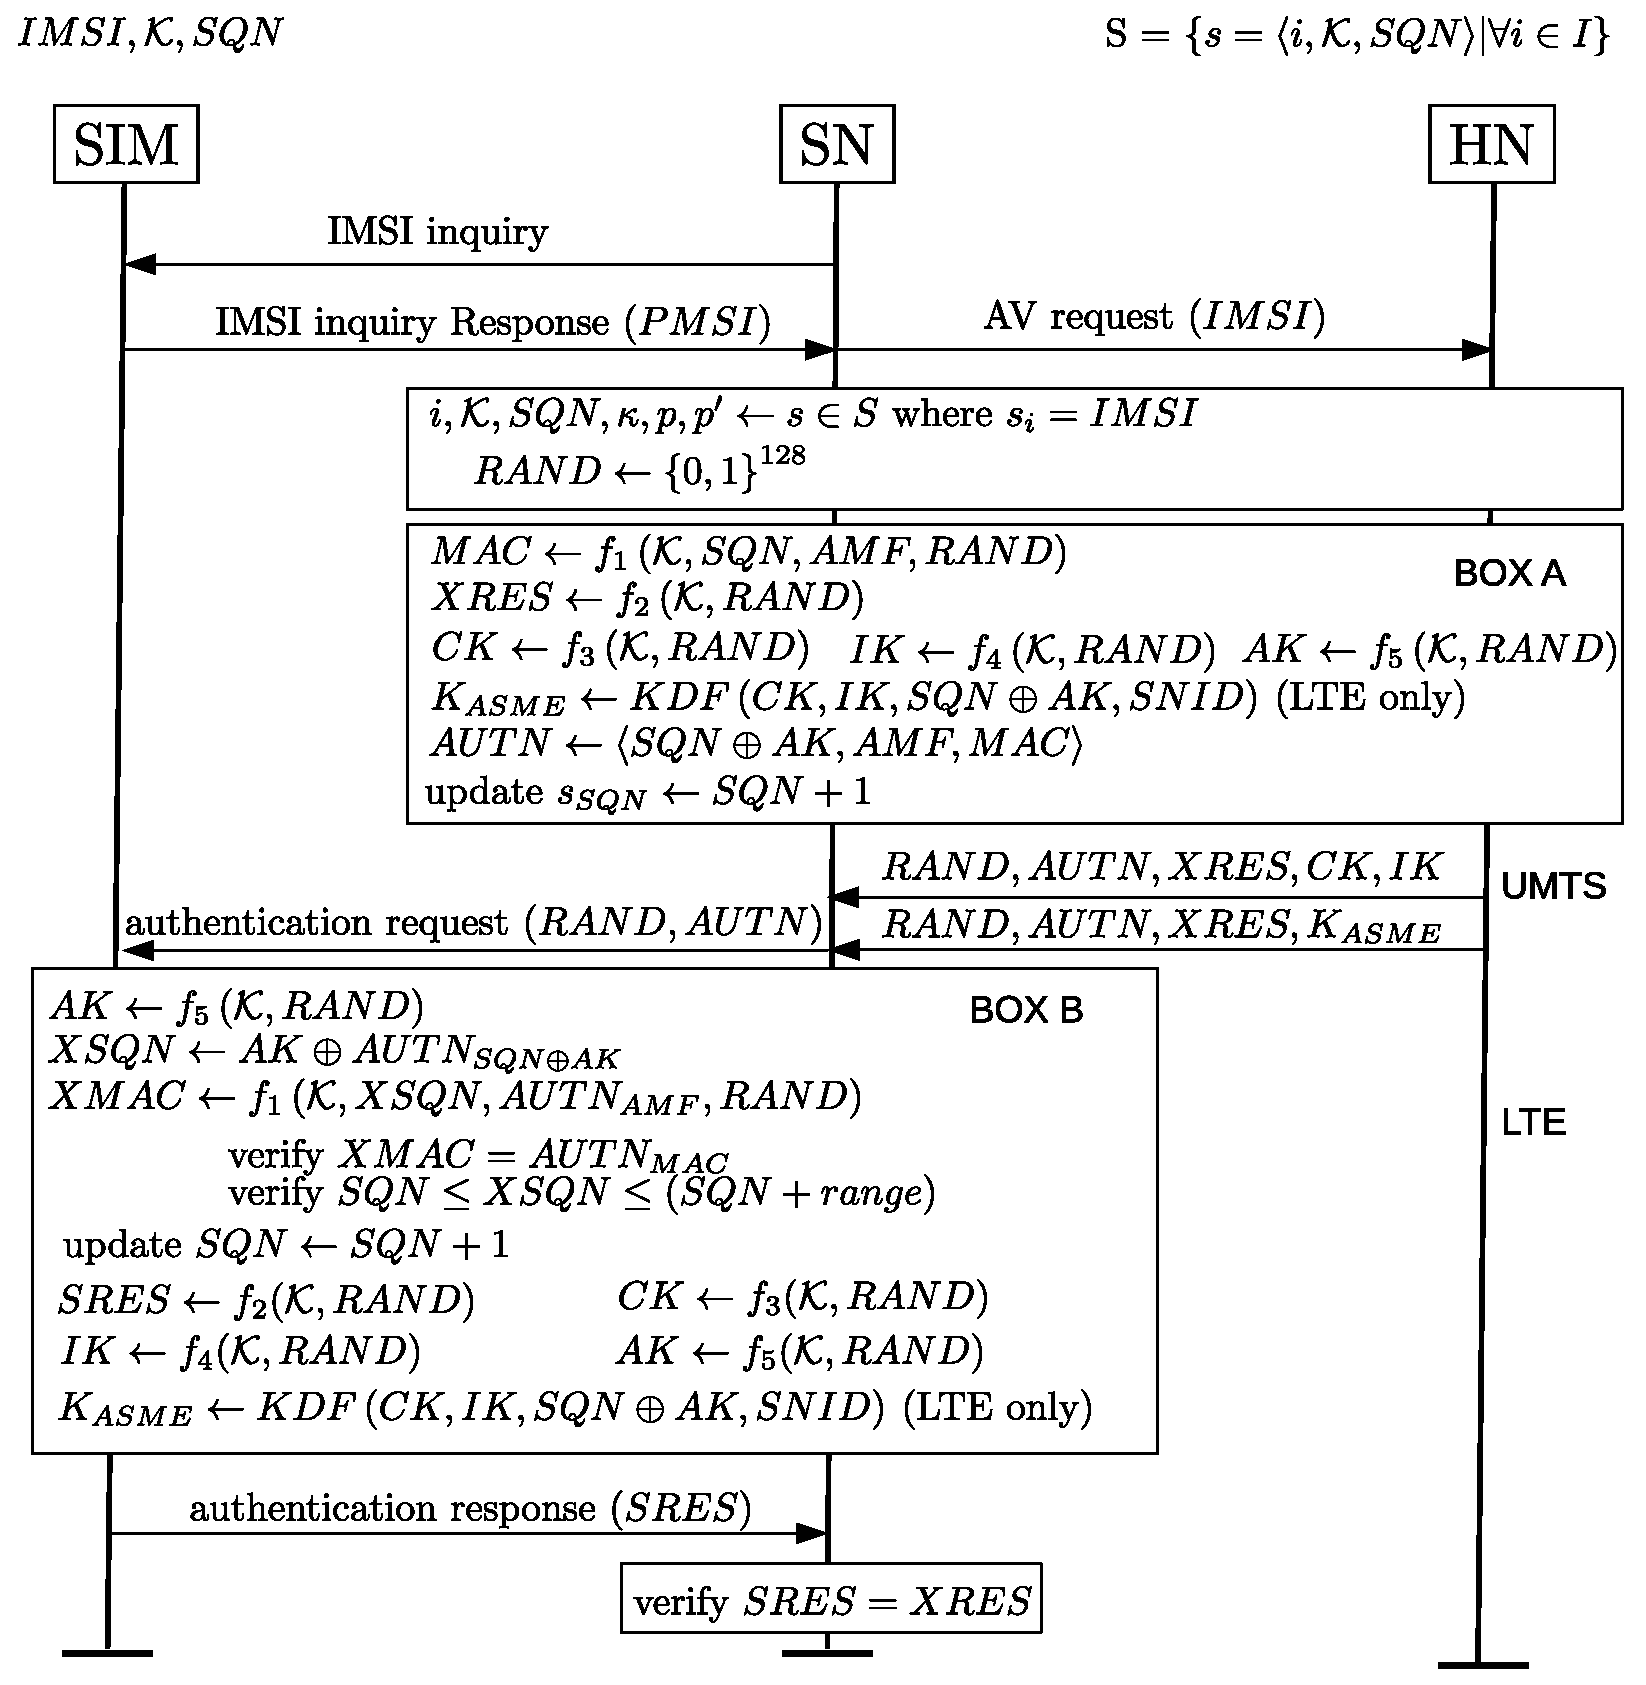
\includegraphics[scale=0.32, clip=true, trim=0cm 0cm 0cm 1cm]{UMTS_LTE_AKA.eps}
  \caption{UMTS/LTE AKA}
  \label{fig:UMTS_LTE_AKA}
\end{figure}

In LTE, upon receiving the AV request, the HN also computes another key $K_{ASME}$. And unlike UMTS, the HN forwards $RAND,AUTN,XRES,K_{ASME}$ to the SN. The UE verifies the $AUTN$, computes $SRES,CK,IK, K_{ASME}$ using the $RAND$ and key $\mathcal{K}$ and forwards $SRES$ to the SN. If $SRES$ and $XRES$ are the same strings, then the authentication is successful. The key $K_{ASME}$ is used to generate further keys for confidentiality and integrity protection. See Figure \ref{fig:UMTS_LTE_AKA}.



\subsection{Location Update} It is specified in 3GPP TS 23.012 (Section 3.6.1.1) \cite{TS23012}, that, when a UE registers with a visitor location register (VLR), an entity in the SN, the  VLR provides its address to the home location register (HLR), an entity in the HN. When a UE uses an IMSI/pseudonym for the first time, it is considered as a registration in the SN and consequently the HN is informed with the address of the SN for the IMSI/pseudonym. We will refer to this location update (LU) message sent for IMSI/pseudonym $x$ as $\texttt{LU}_{x}$ in this paper. We will use these LU messages in our solution.


\section{Related Work}
The BVR and KM schemes describe how the use of HN recognized pseudonym can be introduced in the legacy networks. Also other proposals \cite{Ginzboorg_Niemi_2016,Norrman_Naslund_Dubrova_2016,yemen2017} were published in 2016 and 2017. All these proposals use essentially the same idea of using frequently changing pseudonyms recognized by the HN. The vulnerability identified in \cite{wisec17} is present in all these solutions. We will explain the DDoS attack and our solution in the context of the BVR scheme.

\subsection{BVR Scheme}
Along with the shared secret $\mathcal{K}$, every user shares another secret key $\kappa$ with the HN. The SIM inside the UE stores two pseudonyms at any point of time, $\left(PMSI,P_{new}\right)$. The SIM uses $P_{new}$ the next time the UE receives an IMSI inquiry and keep using $P_{new}$ until it receives a new pseudonym. The HN also stores two pseudonyms $\left(p,p'\right)$ for every users at any point of time. In an ideal situation, $PMSI = p$ and $P_{new} = p'$. 

The HN sends the next pseudonym encrypted by the key $\kappa$ as a part of the random challenge $RAND$ used in AKA. Upon the successful and positive completion of the AKA between the SN and the UE, the next pseudonym can be decrypted by the SIM. The BVR scheme builds on top of the UMTS/LTE AKA. Figure \ref{fig:bvr_solution} shows the required changes. BOX A and BOX B in the figure refer to those operations in the same boxes in Figure \ref{fig:UMTS_LTE_AKA}.


\begin{figure}[]
  \centering
    \includegraphics[scale = .4,clip = true,trim = .1cm 0cm 0cm 0cm]{BVR.eps}
  \caption{The BVR Scheme}
  \label{fig:bvr_solution}	
\end{figure}

Whenever an AV request arrives for $p'$, the HN forgets $p$. Forgetting an old pseudonym is important so that it can be reused. But forgetting before being confirmed that $p'$ has been received by the UE is a vulnerability as pointed in \cite{wisec17}. If a malicious UE identifies itself using a random pseudonym and if by chance, the random pseudonym is associated with a legitimate UE, the HN forgets an old pseudonym for the legitimate UE. In Section \ref{sec:attack} we will show how this vulnerability can be exploited into a fatal DoS attack.


\subsection{KM17 Scheme} \label{sec:km17scheme}
The KM17 scheme uses three pseudonyms at the HN end: $p_{past},p_{current}$ and $p_{future}$. It also uses three recovery identities (RID) : $RID_{past}$, $RID_{current}$ and $RID_{future}$. The $\texttt{LU}_{p_{future}}$ message sent by an SN to an HN after registration of $p_{future}$ is considered as the confirmation that $p_{future}, RID_{future}$ have been delivered to the UE. Upon receiving $\texttt{LU}_{p_{future}}$, the HN forgets $p_{past}$ and $RID_{past}$ by setting $p_{past} \leftarrow p_{current}, p_{current} \leftarrow p_{future}, p_{future} \leftarrow null$ and after some other verifications sets $RID_{past} \leftarrow RID_{current}, p_{current} \leftarrow RID_{future}, RID_{future} \leftarrow null$. The HN always sends $p_{future}$ as the next pseudonym embedded in the AV. If $p_{future}$ is null, it generates an unused new one.


Careful investigation in KM17 scheme shows that a pseudonym has to be used at least two times before the UE can get a new pseudonym from the HN. The HN forgets $p_{past}$ only when $\texttt{LU}_{p_{future}}$ arrives at HN. $\texttt{LU}_{p_{future}}$ would arrive only if $p_{future}$ was used by the UE already at least once. Notice that the $p_{current}$ after arriving $\texttt{LU}_{p_{future}}$ is same as the $p_{future}$ before the $\texttt{LU}_{p_{future}}$ was arrived. And after the arrival of $\texttt{LU}_{p_{future}}$, the $p_{future}$ has become null. So, at this point, to get a new pseudonym, the UE has to use $p_{current}$. Consequently our claim follows. The use of same pseudonym twice happens because the scheme does not forget $p_{past}$ when $\texttt{LU}_{p_{current}}$ arrives. We take care of this issue in our solution.

The authors argue that the scheme is vulnerable to a malicious SN who tries to attack by sending fake LU messages. As a reactive measure, the authors propose a recovery process that enables a UE and the HN to get back in a synchronized state of pseudonyms. The recovery process uses temporary recovery identity (RID). The HN sends the $RID_{future}$ as a part of the $RAND$ in a similar way a pseudonym is sent. When a UE gets convinced that the pseudonym synchronization has been lost, the UE sends the RID piggybacked in the reject message $AUTS$. Based on the RID, the process can recover to a synchronized pseudonym state. Detail of the process can be found in \cite{wisec17}. But, an IMSI catcher can convince a UE that the synchronization has been lost and learn the RID of the UE. After learning the RID, the IMSI catcher can track the user using this RID.

But one might argue that the RIDs can be changed as frequently as the pseudonyms. Note that, forgetting an old RID is also triggered by the same $\texttt{LU}_{p_{future}}$ that triggers forgetting an old pseudonym. Consequently, synchronization of RIDs become as vulnerable as synchronization of pseudonyms, when a malicious SN sends fake LU message. However in the analysis of our solution in Section \ref{sec:analysis}, we will show that a malicious SN can be very quickly detected and stopped before it can mount a meaningful attack.

\section{Attack On BVR Scheme} \label{sec:attack}
The attack is mounted by a malicious UE. The attack has two phases. 

%\subsubsection{Phase 1} \label{sec:attac_fue_phase1}  

\textbf{Phase 1 } A malicious UE sends an attach request using a random pseudonym $q_1$ to a legitimate SN. The legitimate SN sends an AV request for $q_1$ to the HN. If by chance, $q_1 = p'$, the HN forgets $p$ and sets $p \leftarrow p'$. The HN also generates an unused pseudonym $p''$ and sets $p' \leftarrow p^{''}$. As a result, in the HN, the current  pseudonym state for the user $s$ is $\left(p = P_{new},p' \notin \left\lbrace PMSI,P_{new} \right\rbrace \right)$. %See Figure \ref{fig:dos_attack}.

%\subsubsection{Phase 2} \label{sec:attac_fue_phase2} 
\textbf{Phase 2 }The malicious UE sends another attach request using a random pseudonym $q_2$ to a legitimate SN. The legitimate SN sends a AV request for $q_2$ to the HN. If again by chance, $q_2 = p'$, then the HN again forgets $p$, sets $p \leftarrow p'$. HN also generates an unused pseudonym $p'''$ and sets $p' \leftarrow p'''$. Consequently, the current pseudonym state of user $s$ is $\left\lbrace PMSI,P_{new} \right\rbrace \cap \left\lbrace p,p' \right\rbrace = \emptyset$. %See Figure \ref{fig:dos_attack}

%\begin{figure}[]
%  \centering
%    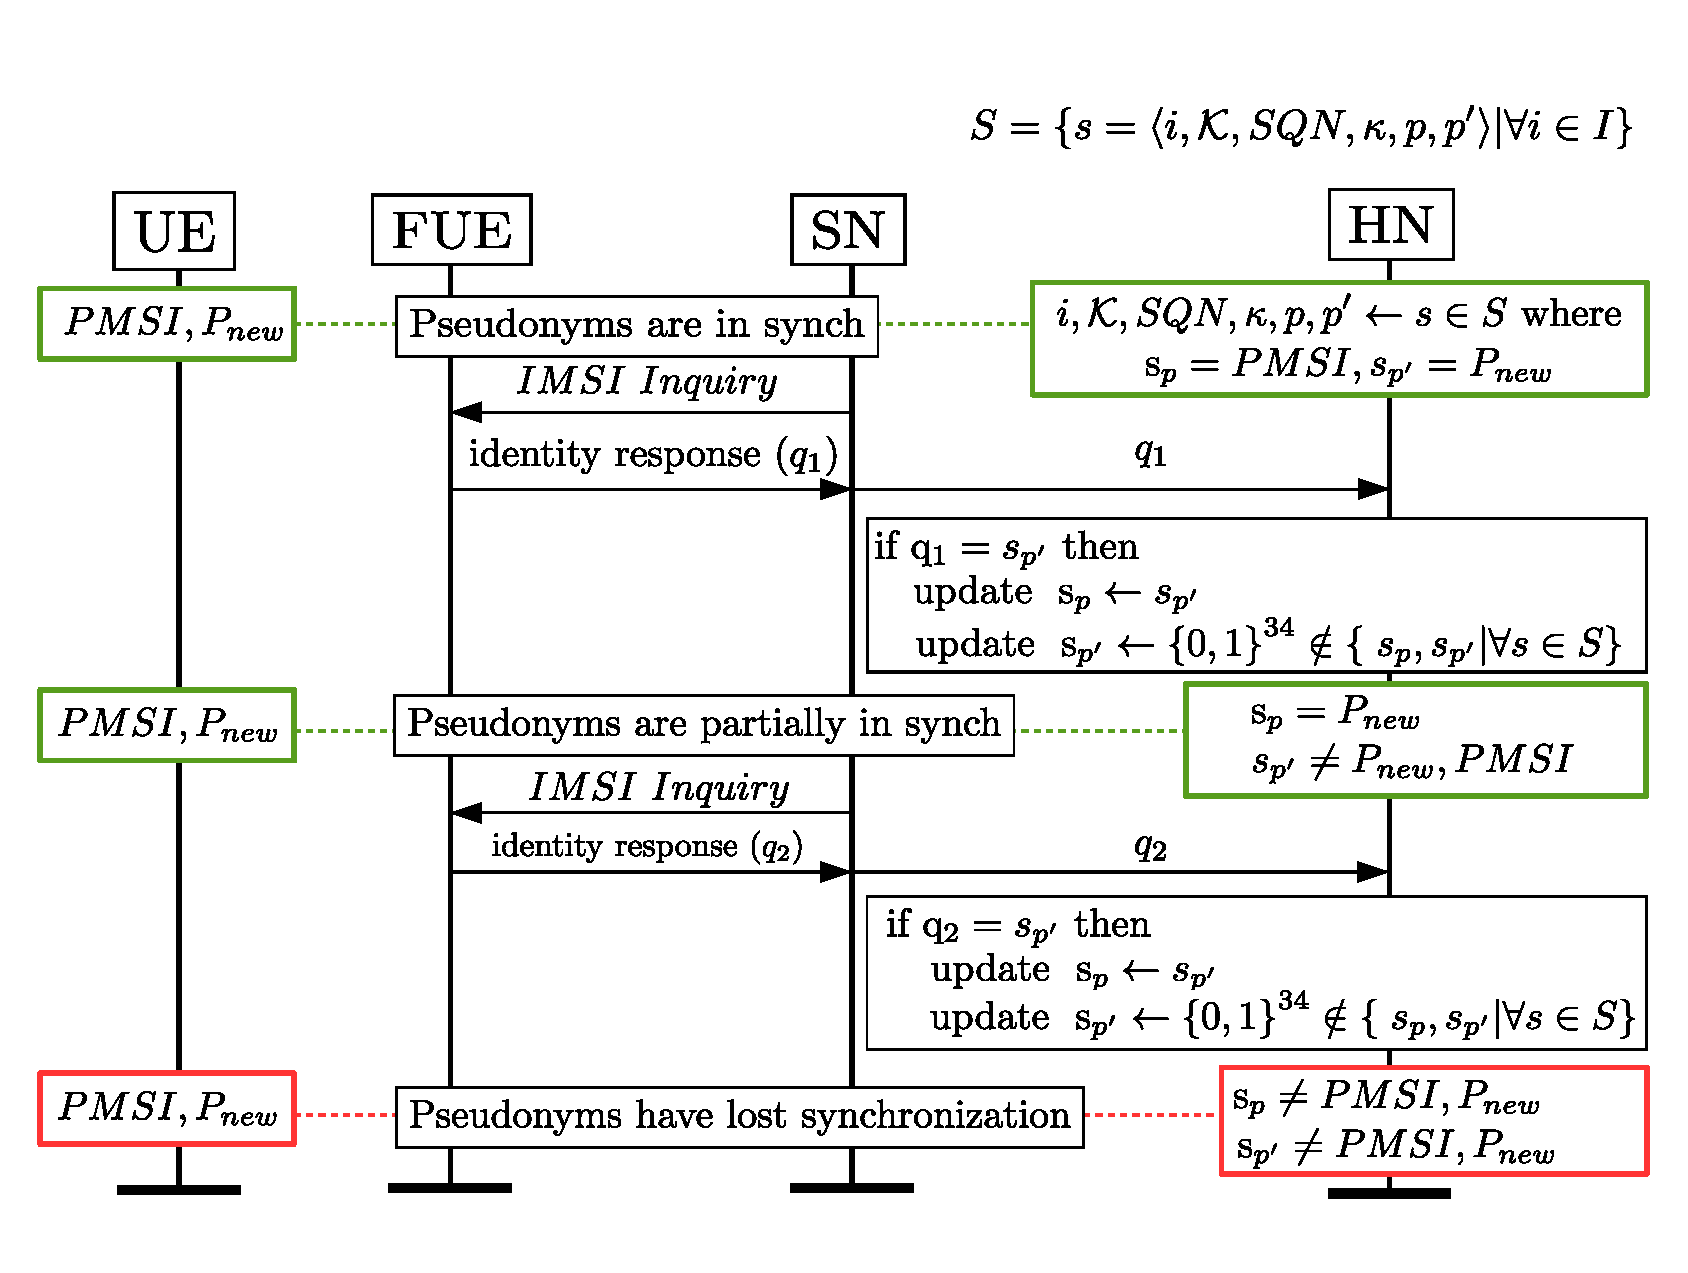
\includegraphics[width=.9\textwidth]{DDoS.eps}
%  \caption{A DoS Attack against the BVR scheme}
%  \label{fig:dos_attack}	
%\end{figure}

The next time the user would need to authenticate itself to a network, the authentication will fail and hence be denied any service. In this attack, it is assumed that the UE has not obtained a new pseudonym via a legitimate SN while the attack was mounted.

\subsection{The DDoS Attack Against the BVR Scheme} \label{sec:ddos_attack}
The DDoS attack is mounted by a botnet of mobile devices. The mobile bots send many attach requests using different pseudonyms to legitimate SNs. The legitimate SNs in turn sends AV request for those pseudonyms to the HN. Let us assume, the total number of pseudonyms sent to the HN is a large integer $m$. In this case, a user $s$ will be affected by the attack if there exists two integers $0 < x < y \leq m$ such that $q_{x} = p'$ and $q_{y} = p'$. 


We have considered two different ways to mount this attack. In one way, the pseudonyms used in the attach requests are chosen randomly with replacement, which means the attack might sent one pseudonym more than once to the HN. In the other way, the pseudonyms are chosen without replacement, which means the attack send one pseudonym only once.

\textbf{With Replacement:} In this case, after sending $m$ number of pseudonyms to the HN, the expected portion of affected users $E[u_a]$ is
\begin{eqnarray}
E\big[ u_a \big] &=& 1- \left(1 - \frac{1}{\mathcal{M}}\right)^m - m\left(\frac{1}{\mathcal{M}}\right)\left(1 - \frac{1}{\mathcal{M}}\right)^{\left(m-1 \right)} \label{eqn:avg_with_replacement}
\end{eqnarray} 
See the derivation in Appendix \ref{appendix:A}.  We have run a simulation of this attack and found that above model is fairly accurate. See Figure \ref{fig:simulation_and_modeling}.


\begin{figure}[]
  \centering
  \begin{minipage}[b]{0.49\textwidth}
    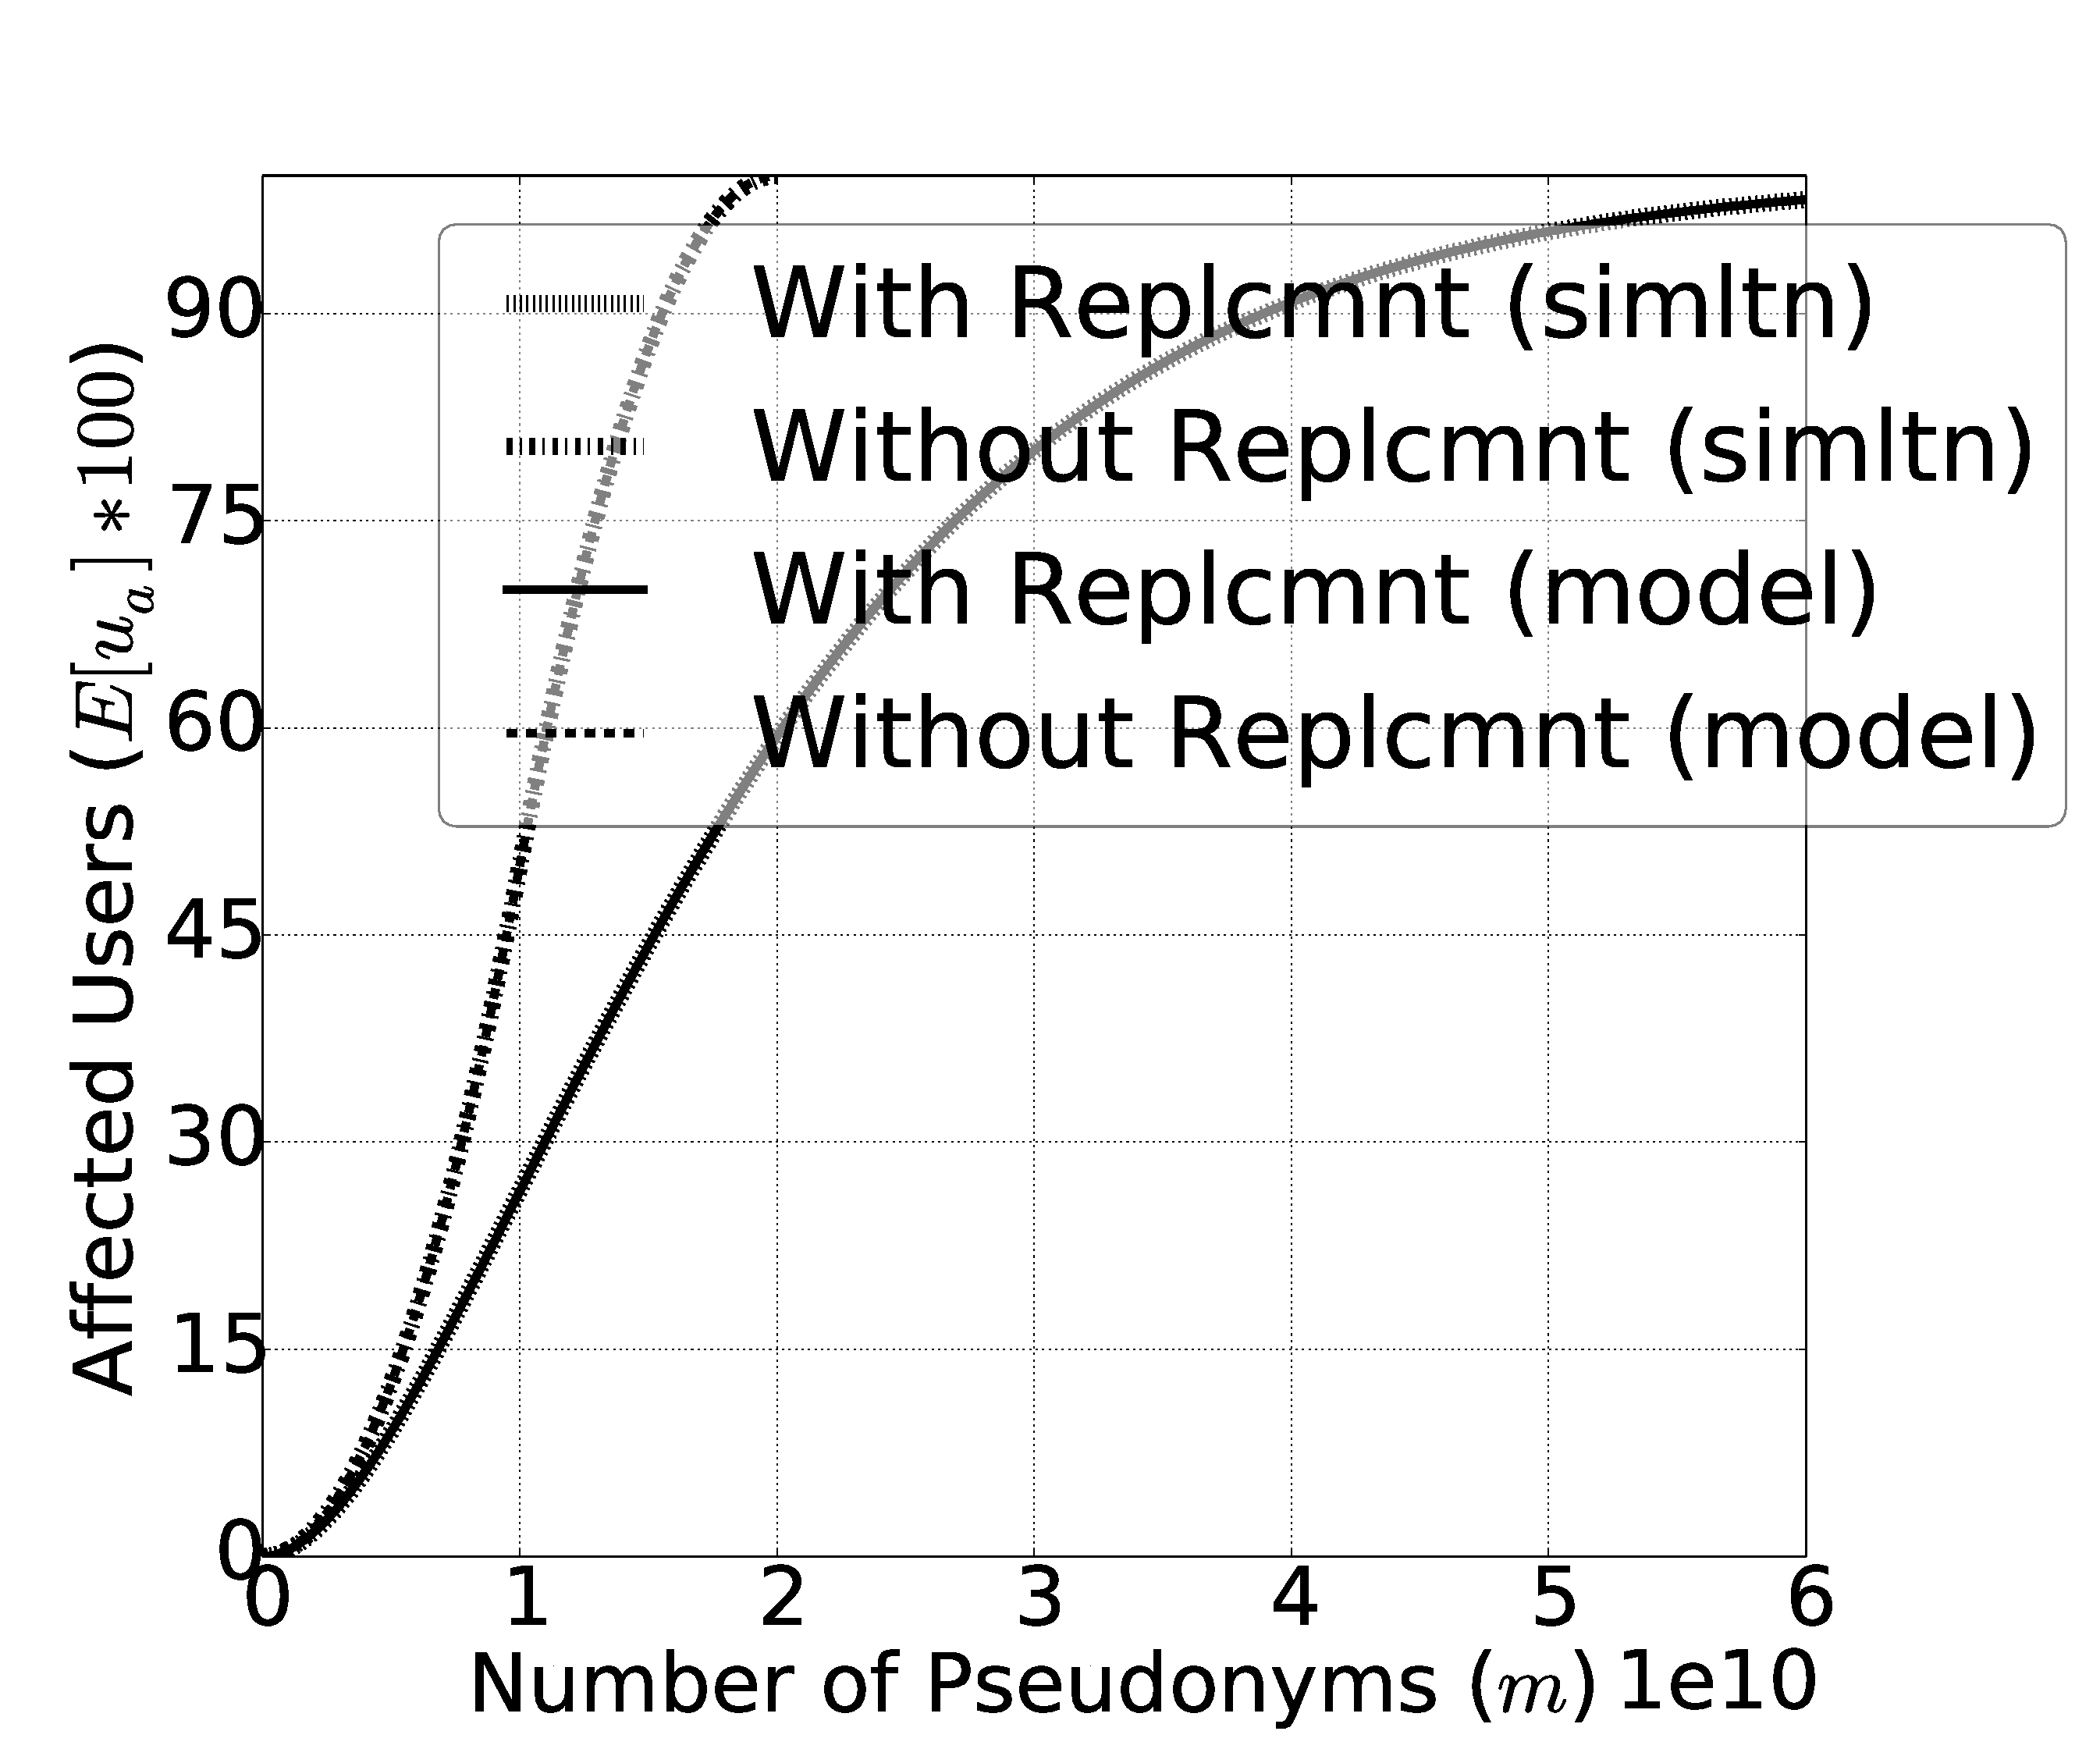
\includegraphics[width=\textwidth]{sim_and_mod.pdf}
   \caption{DDoS Attack. $ \mathcal{M} = 10^{10}, n = 10^{7}$. The model fits so well that it is difficult to distinguish the empirical lines from the model.}
\label{fig:simulation_and_modeling}
  \end{minipage}

  \hfill
  \begin{minipage}[b]{0.49\textwidth}
    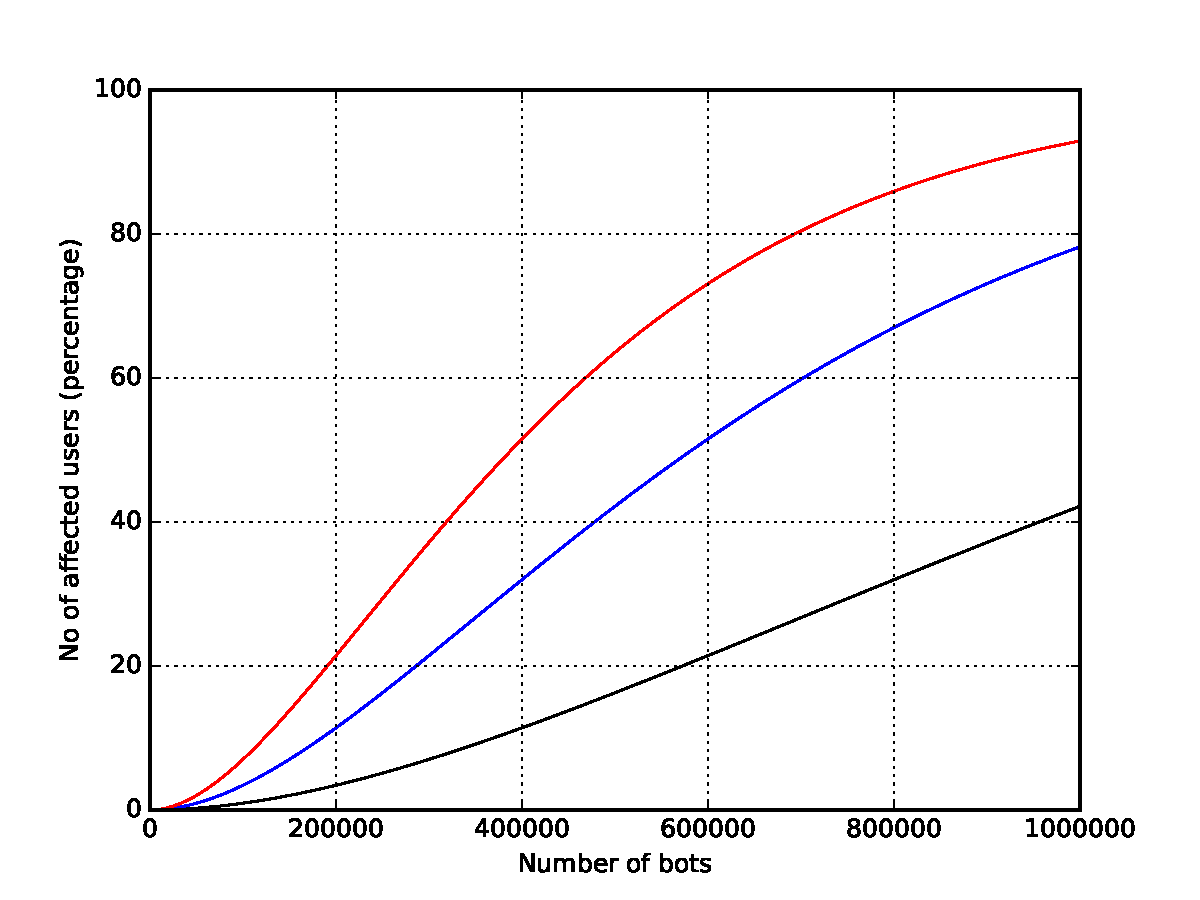
\includegraphics[width=\textwidth]{botplot.pdf}
    \caption{DDoS Attack (with replacement), $\texttt{botnet}_{\texttt{size}} = 10^6$. Different lines represent the success rate as $\texttt{bot}_{\texttt{load}}$ varies.}
  \label{fig:botplot}
  \end{minipage}
\end{figure}

\textbf{Without Replacement:} In this case the attacker runs two rounds of the attack. In the first round the attacker sends all the pseudonyms in the IMSI space without replacement, means each pseudonym is sent exactly once. Once the first round is completed, the attacker runs the attack for one more round. However, after sending $m$ number of pseudonyms to the HN, the expected
 portion of affected users $E[u_a]$ is
\begin{eqnarray}
E\big[ u_a \big] = \begin{cases} \frac{m^2}{2\cdot \mathcal{M}^2} & \mbox{if } 0 < m \leq \mathcal{M} \\ 
\frac{1}{\mathcal{M}}(2m - \mathcal{M} - \frac{m^2}{2\mathcal{M}}) & \mbox{if } \mathcal{M} < m \leq 2\mathcal{M} \end{cases}
\label{eqn:without_replacement}
\end{eqnarray} 

See the derivation in Appendix \ref{appendix:B}. We have run a simulation of this attack and found that above model is fairly accurate. See Figure \ref{fig:simulation_and_modeling}. Note that, this is an estimation where the without-replacement attack is not a distributed attack. Rather the attack is mounted by only a single malicious UE. In the case of distributed and without replacement attack, the expected percentage of affected users will be less than what is shown in the plot. However, we believe that, the distributed and without replacement attack will have higher number of affected users than that of distributed with replacement attack. %However, it can be a strategic decision of the attacker to choose the value of $\texttt{bot}_{\texttt{load}}$.


\subsection{How Fatal The DDoS Attack Can be In Practice} \label{sec:how_fatal_ddos}
The intensity of the attack will depend on the size of the botnet and number of pseudonyms send by one bot in a unit time. We name these parameters as $\texttt{botnet}_{\texttt{size}}$ and $\texttt{bot}_{\texttt{load}}$ respectively. According to \cite{thesislund}, the EPS AKA has the latency of $550$ milliseconds. So, the peak value of $\texttt{bot}_{\texttt{load}}$ can safely be considered as $1$ pseudonyms/second, i.e., 3600 pseudonyms/hour.

Mobile botnets are on the rise \cite{botnet_ccs09_symbian,botnet_usenix11,botnet_australia_2016}. Many mobile botnets have already been observed, e.g., Geinimi \cite{botnet_geinimi10}, Zeus \cite{botnet_zeus11}, AnserverBot \cite{botnet_anserverbot}, DreamDroid \cite{botnet_dreamdroid11}. A detailed survey of the state of mobile botnets can be found in \cite{botnet_threat15}. In 2011, it was estimated that Dreamdroid was installed on 120,000 mobile devices \cite{botnet_dreamdroid11}. In 2014, a mobile botnet of 650,000 mobile phones made an attack to a server \cite{chinese_spam}. It would not be surprising if we see a mobile botnet consisting tens of millions of mobile bots in near future. However, for the discussion of this paper, we conservatively set the variable $\texttt{botnet}_{\texttt{size}} = 1$ million ($10^6$). See Figure \ref{fig:botplot}, it shows how efficient a botnet of size $10^6$ can be for varied values of $\texttt{bot}_{\texttt{load}}$.



\section{Our Solution}
In the HN, for a user $s$, our solution stores the IMSI $i$ and three pseudonyms $p,p',p''$. In the SIM of the user $s$, two pseudonyms $PSMI,P_{new}$ are stored. In an ideal situation $PMSI = p, P_{new} = p'$. We build our solution on top of the BVR and KM17 scheme. The pseudonyms $p,p',p''$ can be compared with $p_{past},p_{current},p_{future}$ of KM17 scheme. However, unlike KM17 scheme, our solution uses $\texttt{LU}_{p'}$ to forget $p$. Let us assume that for a user $s$ an AV request has arrived using the pseudonym $p$ and the HN has responded with an AV by embedding $p'$ in the $RAND$. When an LU for pseudonym $p$ arrives, the HN considers it as the guarantee that pseudonym $p'$ has been delivered to the UE of user $s$.  Figure \ref{fig:solution} presents our solution. The bold texts present the changes over UMTS/LTE AKA. BOX A and BOX B in the figure refer to those operations in the same boxes in Figure \ref{fig:UMTS_LTE_AKA}.

\begin{figure}[]
  \centering
    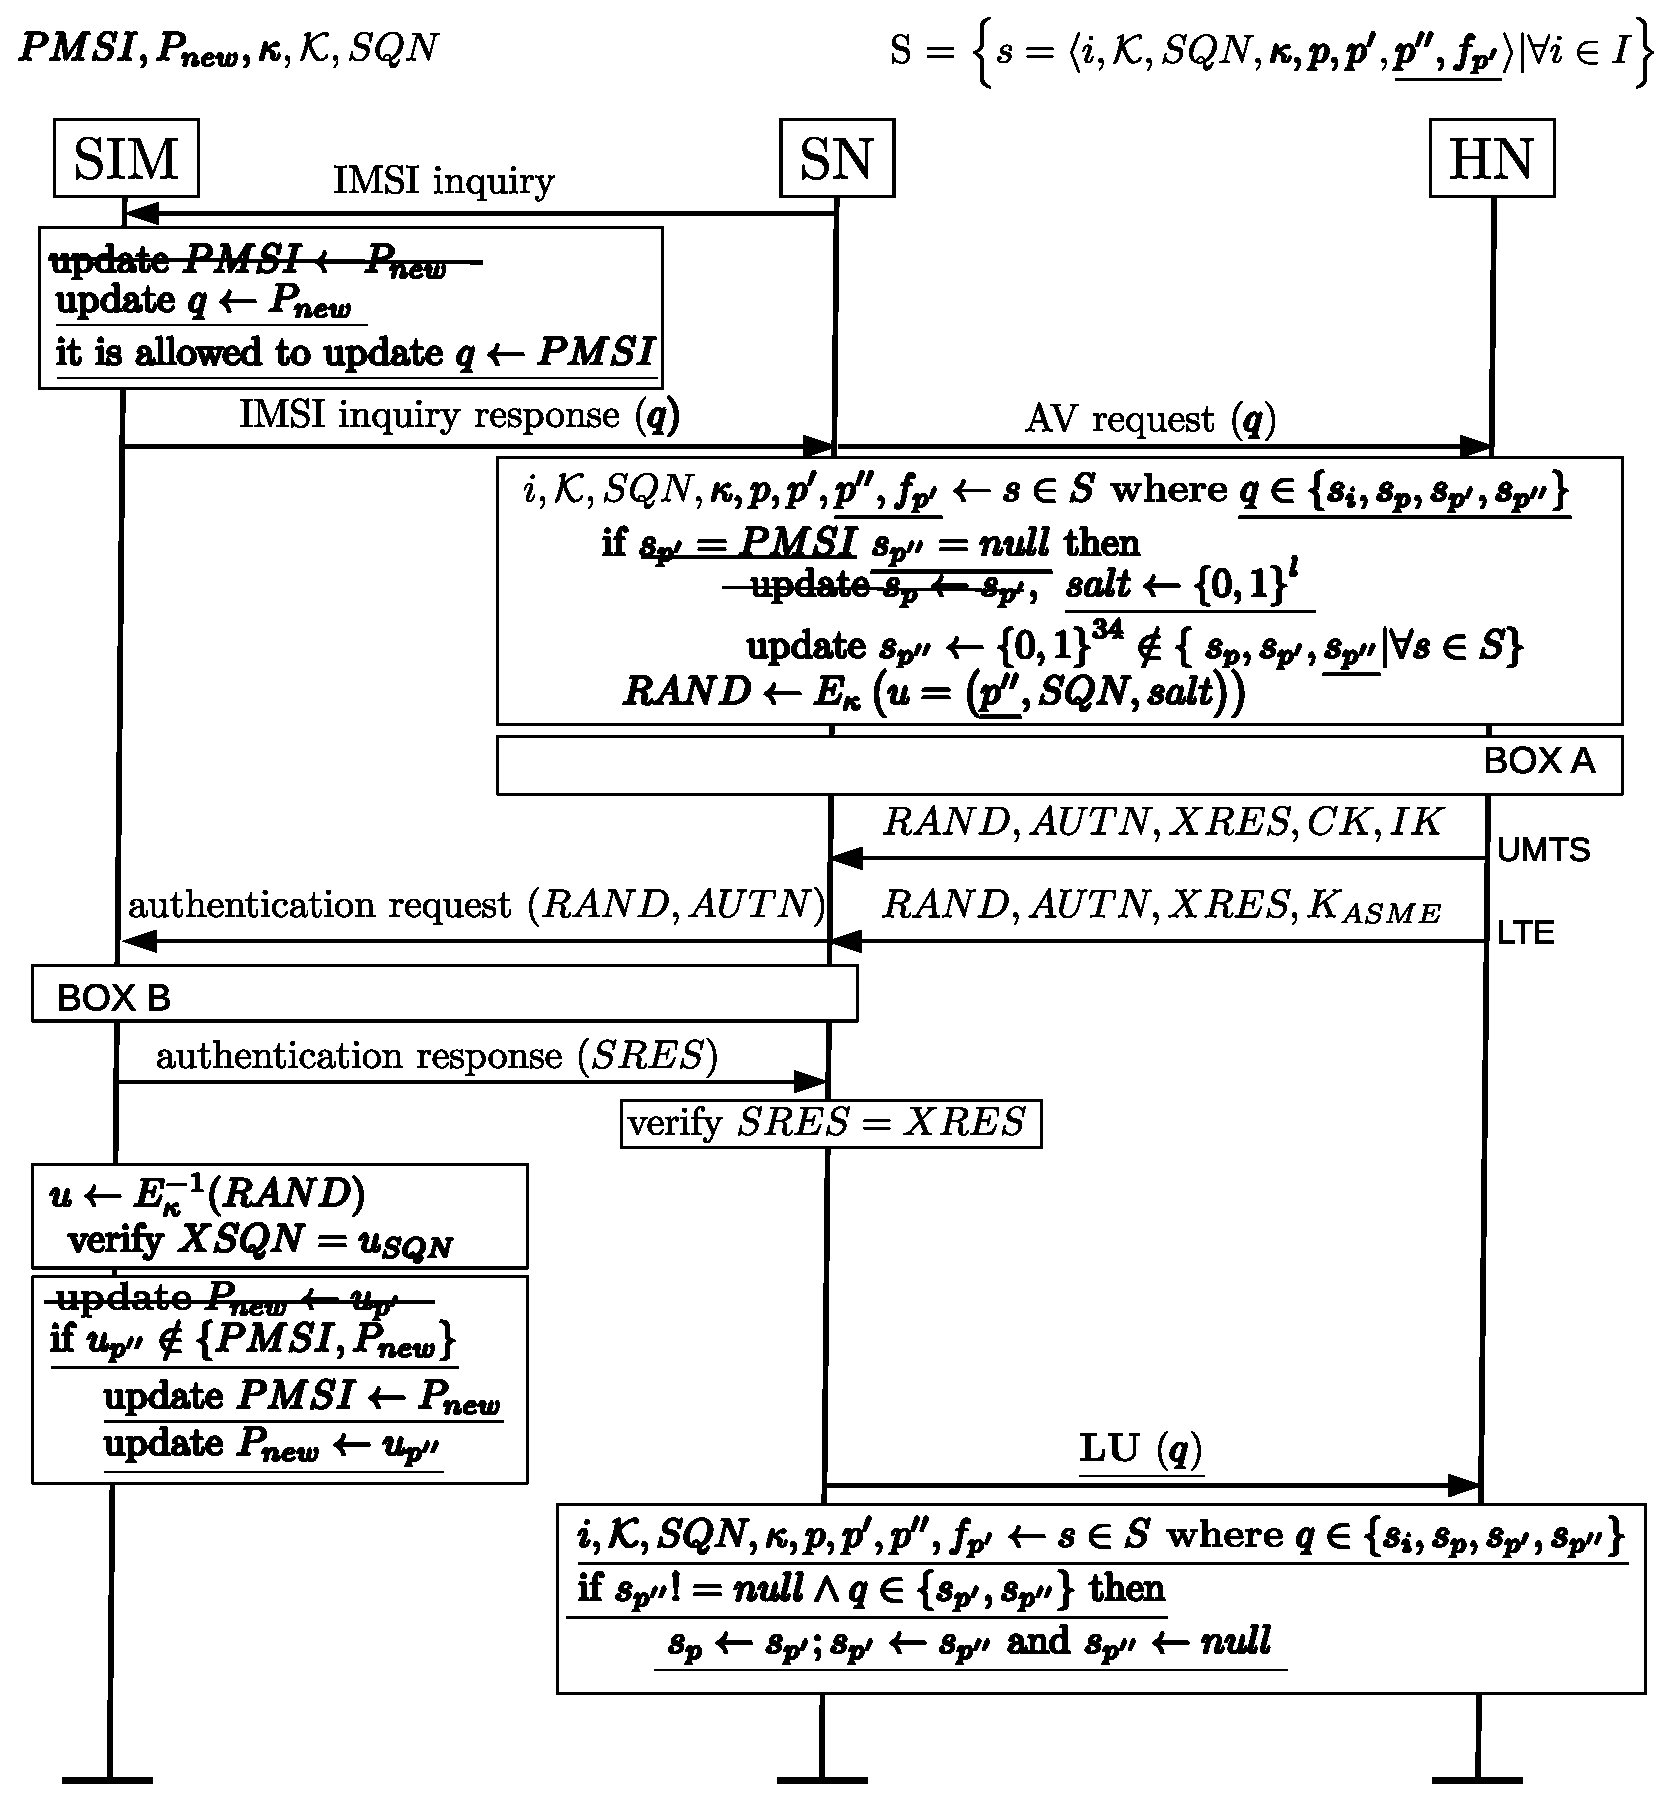
\includegraphics[scale = .38,clip = true, trim = 0cm 0cm 0cm 0cm]{solution.eps}
  \caption{Solution}
  \label{fig:solution}	
\end{figure}

\textbf{At HN side } Whenever an AV request is received for a user $s$, using any of its identity, i.e., $i,p,p'$ or $p''$, the HN responds with an AV that contains the pseudonym $p''$ in the $RAND$. If $p''$ is $null$ then an unused pseudonym is chosen and set as $p''$. When $p''$ is not null and LU message $\texttt{LU}_{p'}$ or $\texttt{LU}_{p''}$ arrives, the HN forgets $p$ by setting $p \leftarrow p', p' \leftarrow p''$ and $p'' \leftarrow null$. 

\textbf{At UE side } During the AKA, if $MAC$ and $SEQN$ verification is successful then the UE sends the $SRES$ to the SN. Then the UE verifies if $u_{SEQN}$ is the same as the $XSEQN$. See Figure \ref{fig:solution}. If this verification is also successful and $u_{p''} \notin \left\lbrace PMSI,P_{new} \right\rbrace$, then the UE sets $PMSI \leftarrow P_{new}$ and $P_{new} \leftarrow u_{p''}$. After a successful AKA the old pseudonym $PMSI$ will still be used in place of permanent identity IMSI by the current SN, for example, in paging messages, and in subsequent communications between an HN and an SN. The identity $P_{new}$ comes into play in the next SN. 

However, it is upon the freedom of the UE to identify itself either with $PMSI$ or $P_{new}$ in an attach request or in response to an IMSI inquiry. If the consequent AKA fails many times after identifying with $PMSI$, the UE would identify itself using $P_{new}$.


\section{Analysis of Our Solution} \label{sec:analysis}
LU messages maybe delayed, lost, or sent multiple times. Also in practice, the LU messages $\texttt{LU}_p,\texttt{LU}_{p'},\texttt{LU}_{p''}$ might arrive in different order because of the inherent characteristics of IP networks. A malicious or faulty SN might send a LU message even when the corresponding AKA was failed or maybe not even run. To understand, how our solution behaves in these unusual but possible situations, we study different categories of states a user $s$ can be in the HN or the UE, based on the relevant variables and eventually construct a global state diagram of our solution. Based on the global state diagram we show how our solution behaves in different situations.

\subsection{State Diagrams}
We divide all the possible states of a user $s$ in HN in two categories. The first category is the one where $p''$ is not null and the second category is the one where $p''$ is null. Based on these two categories, we draw a state diagram as presented in Figure \ref{fig:HN_UE_diagrams} (right side). The notation used below is explained in the lower part of Figure 6. Note that our solution is not sensitive to $\texttt{LU}_{i}$ and $\texttt{LU}_{p}$. Consequently only $\texttt{LU}_{p'}$ and $\texttt{LU}_{p''}$ are shown in the diagram.

On the other hand, the UE has only one kind of states as shown in Figure \ref{fig:HN_UE_diagrams} (left side). It always has two pseudonyms $PMSI, P_{new}$. However, $PMSI$ and $P_{new}$ may have different values. The values of $PMSI,P_{new}$ may change only when a successful AKA happens. For a user $s$, we have excluded the possibility of  $\texttt{AKA($x,y$)}$ where $x \notin \left\lbrace PMSI,P_{new} \right\rbrace$ because the UE will receive a wrong $RAND$ in that case. We also have excluded the possibility of $\texttt{AKA($x,y$)}$ where $y \notin \left\lbrace p,p',p'' \right\rbrace$. The reason for this exclusion is discussed in detail in Section \ref{sec:analysis}. According to our solution, the UE does not do anything when $\texttt{AKA($x,y$)}$ happens where $y \in \left\lbrace PMSI,P_{new} \right\rbrace$. However, even if $\texttt{AKA($PMSI,y$)}$ happens where $y \notin  \left\lbrace PMSI,P_{new} \right\rbrace$, the UE does not forget $PMSI$ because $PMSI$ would still be used by the SN, e.g., in paging messages. Consequently only $\texttt{AKA}(P_{new},y)$ where $y \notin  \left\lbrace PMSI,P_{new} \right\rbrace$ is shown in the diagram.


Next we merge the state diagrams of HN and UE into a global state diagram of our solution (Figure \ref{fig:solution_diagram}). The state of user's pseudonyms in the system can be described by whether $PMSI$ and $P_{new}$ on the UE side are one of $p, p', p''$ or not, and by whether in the HN $p''$ has been allocated for user s or not. Based on this description, there can be $4\cdot4\cdot2 = 32$ pseudonyms-state of a user. But many of the states are never reachable. For example, it can never happen that $PMSI$ and $P_{new}$ in the UE are the same because a UE forgets $PMSI$ only if the new pseudonym $p''$ is not in the set $\left\lbrace PMSI,P_{new} \right\rbrace$. All the inputs that can cause a transition of from one state to another in the state diagrams of HN and UE can also cause a transition from one state to another in the global state diagram (Figure \ref{fig:solution_diagram}). 

In our solution, it is assumed that the initial state of a user in the system is $PMSI=p, P_{new}=p'$ on the UE side, and $p''$ has been allocated in the HN. Taking into account the possible transitions, we have found out that only $10$ out of $32$ possible states are reachable from this initial state. Those $10$ states are illustrated in Figure \ref{fig:solution_diagram}. Note that neither the UE nor the HN has the knowledge in which state a user $s$ is in the global diagram. All a UE knows are two pseudonyms $PMSI,P_{new}$ and the HN knows three pseudonyms $p,p',p''$. 

For the limitation of space, we are not going to discuss all the states. Nevertheless, to assist the readers in understanding the diagram, let us take a closer look in few transitions. Let us consider that the user is currently at State $1$. Since, $p''$ is already allocated, $\texttt{AVR}$ has no impact on this state. Consequently we do not mention $\texttt{AVR}$ in this state. Since $p''$ is allocated, it is possible that $\texttt{AKA}(P_{new},p'')$ may run. If either one of these two AKAs happen, the UE forgets PMSI. Such an AKA run has no impact in HN until it receives the corresponding LU. Hence, the user moves to State $2$ in the solution diagram where $PMSI = p', P_{new} = p'', p'' \neq null$. However, while at State $1$, if either one of the LU messages $\texttt{LU}_{p'}, \texttt{LU}_{p'}$ arrives in the HN, the HN forgets $p$. Hence, the user goes to State $4$ in the diagram where $PMSI \notin \left\lbrace p,p',p'' \right\rbrace, P_{new} = p, p'' = null$. The AV request $\texttt{AVR}$ can cause a transition only when $p''=null$, e.g., State $4$.

Observe that the pseudonyms in UE and HN are (i) synchronized in states $1$-$3$; (ii) partially unsynchronized in states $4$, $5$, $7$, $8$ and $9$; (iii) completely unsynchronized in states $6$ and $10$, without any possibility of automatic recovery.


%Based on successful AKA in between the UE and the SN, the values of $PMSI, P_{new}$ may change in the UE. On the other hand, the values of $p,p',p''$ may change due to the arrival of an AV request or a LU message at HN. The action taken by an HN upon receiving an AV request or an LU message depends on the value of $p''$ (null or not null). Figure \ref{fig:solution_diagram} shows the state diagram of our solution with $10$ reachable states out of the total $32$. Notations in Figure \ref{fig:HN_UE_diagrams} are also applicable in Figure \ref{fig:solution_diagram}. In Figure \ref{fig:solution_diagram}, we have excluded the possibility of running an $\texttt{AKA($x,y$)}$ where $x \in \left\lbrace p,p',p^{''} \right\rbrace, y \notin \left\lbrace p,p',p^{''} \right\rbrace$. In Section \ref{sec:replay_attack_sn}, we argue why it is not feasible even when a malicious SN tries to mount a replay attack. 


\begin{figure}
\centering
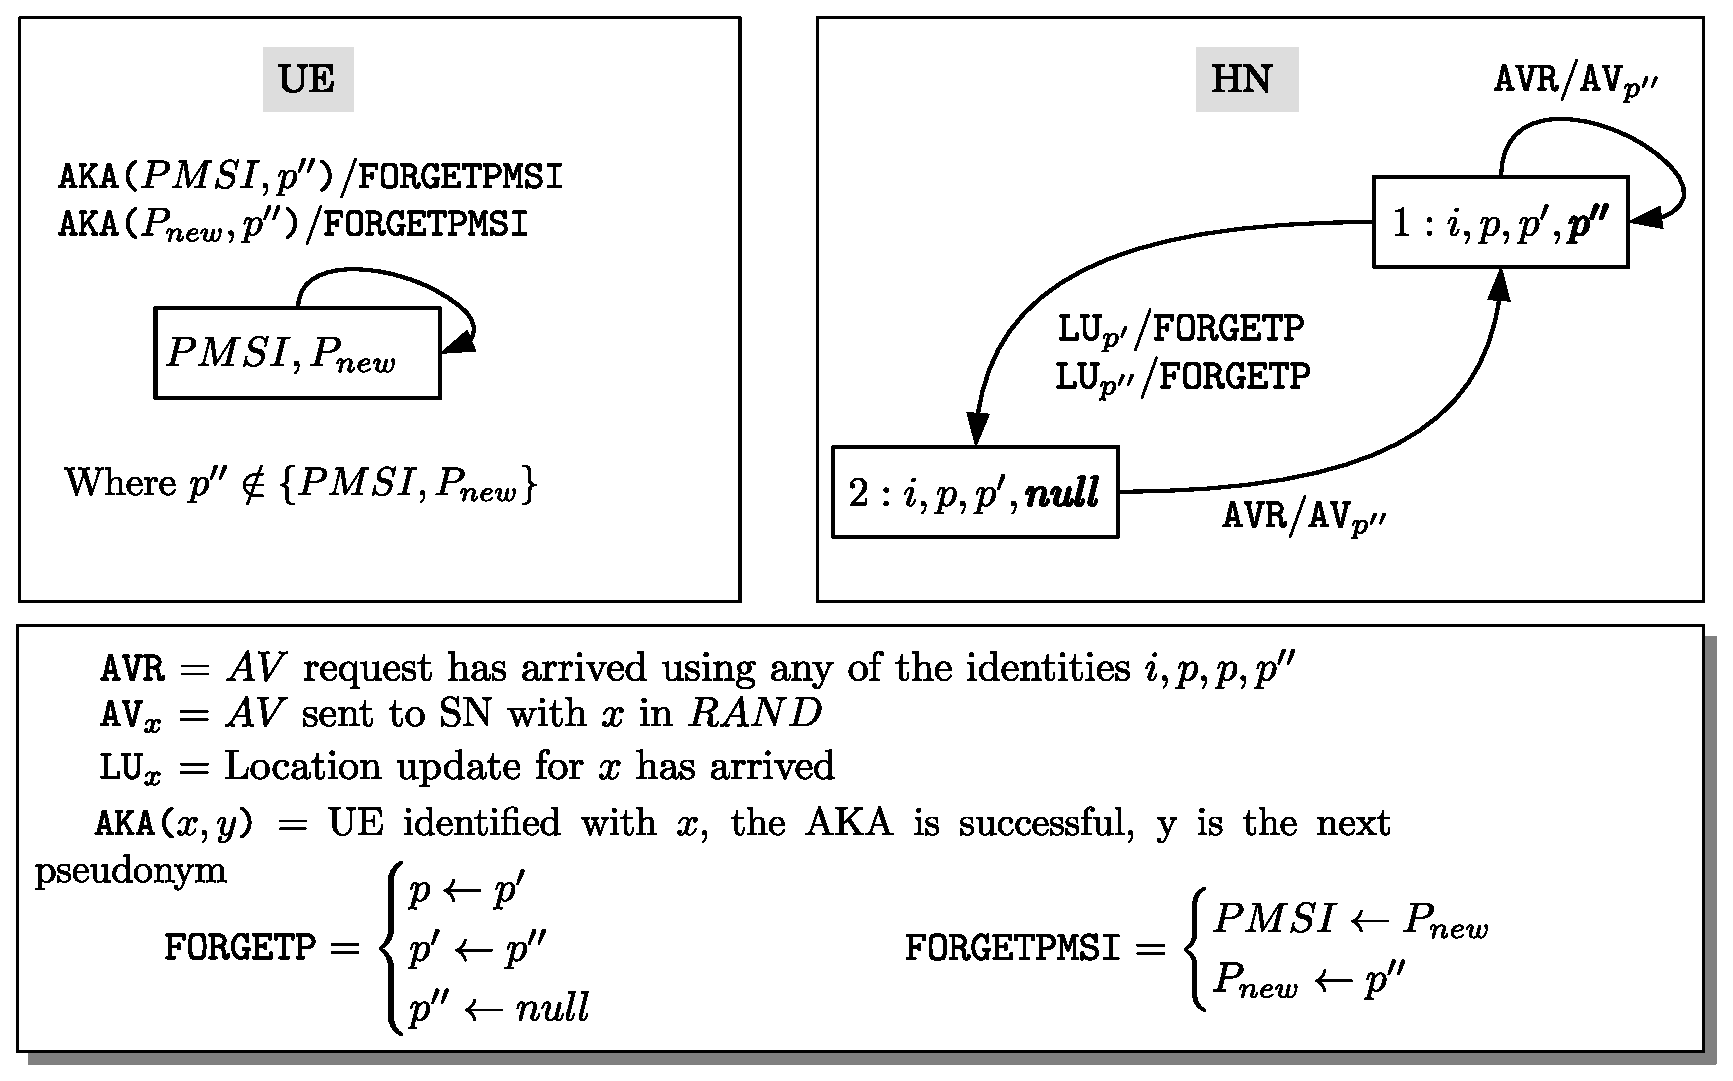
\includegraphics[scale = .4]{HN_UE_diagrams.eps}
\caption{State diagrams of UE and HN}
\label{fig:HN_UE_diagrams}
\end{figure}



\begin{figure}[!tbp]
  \centering
    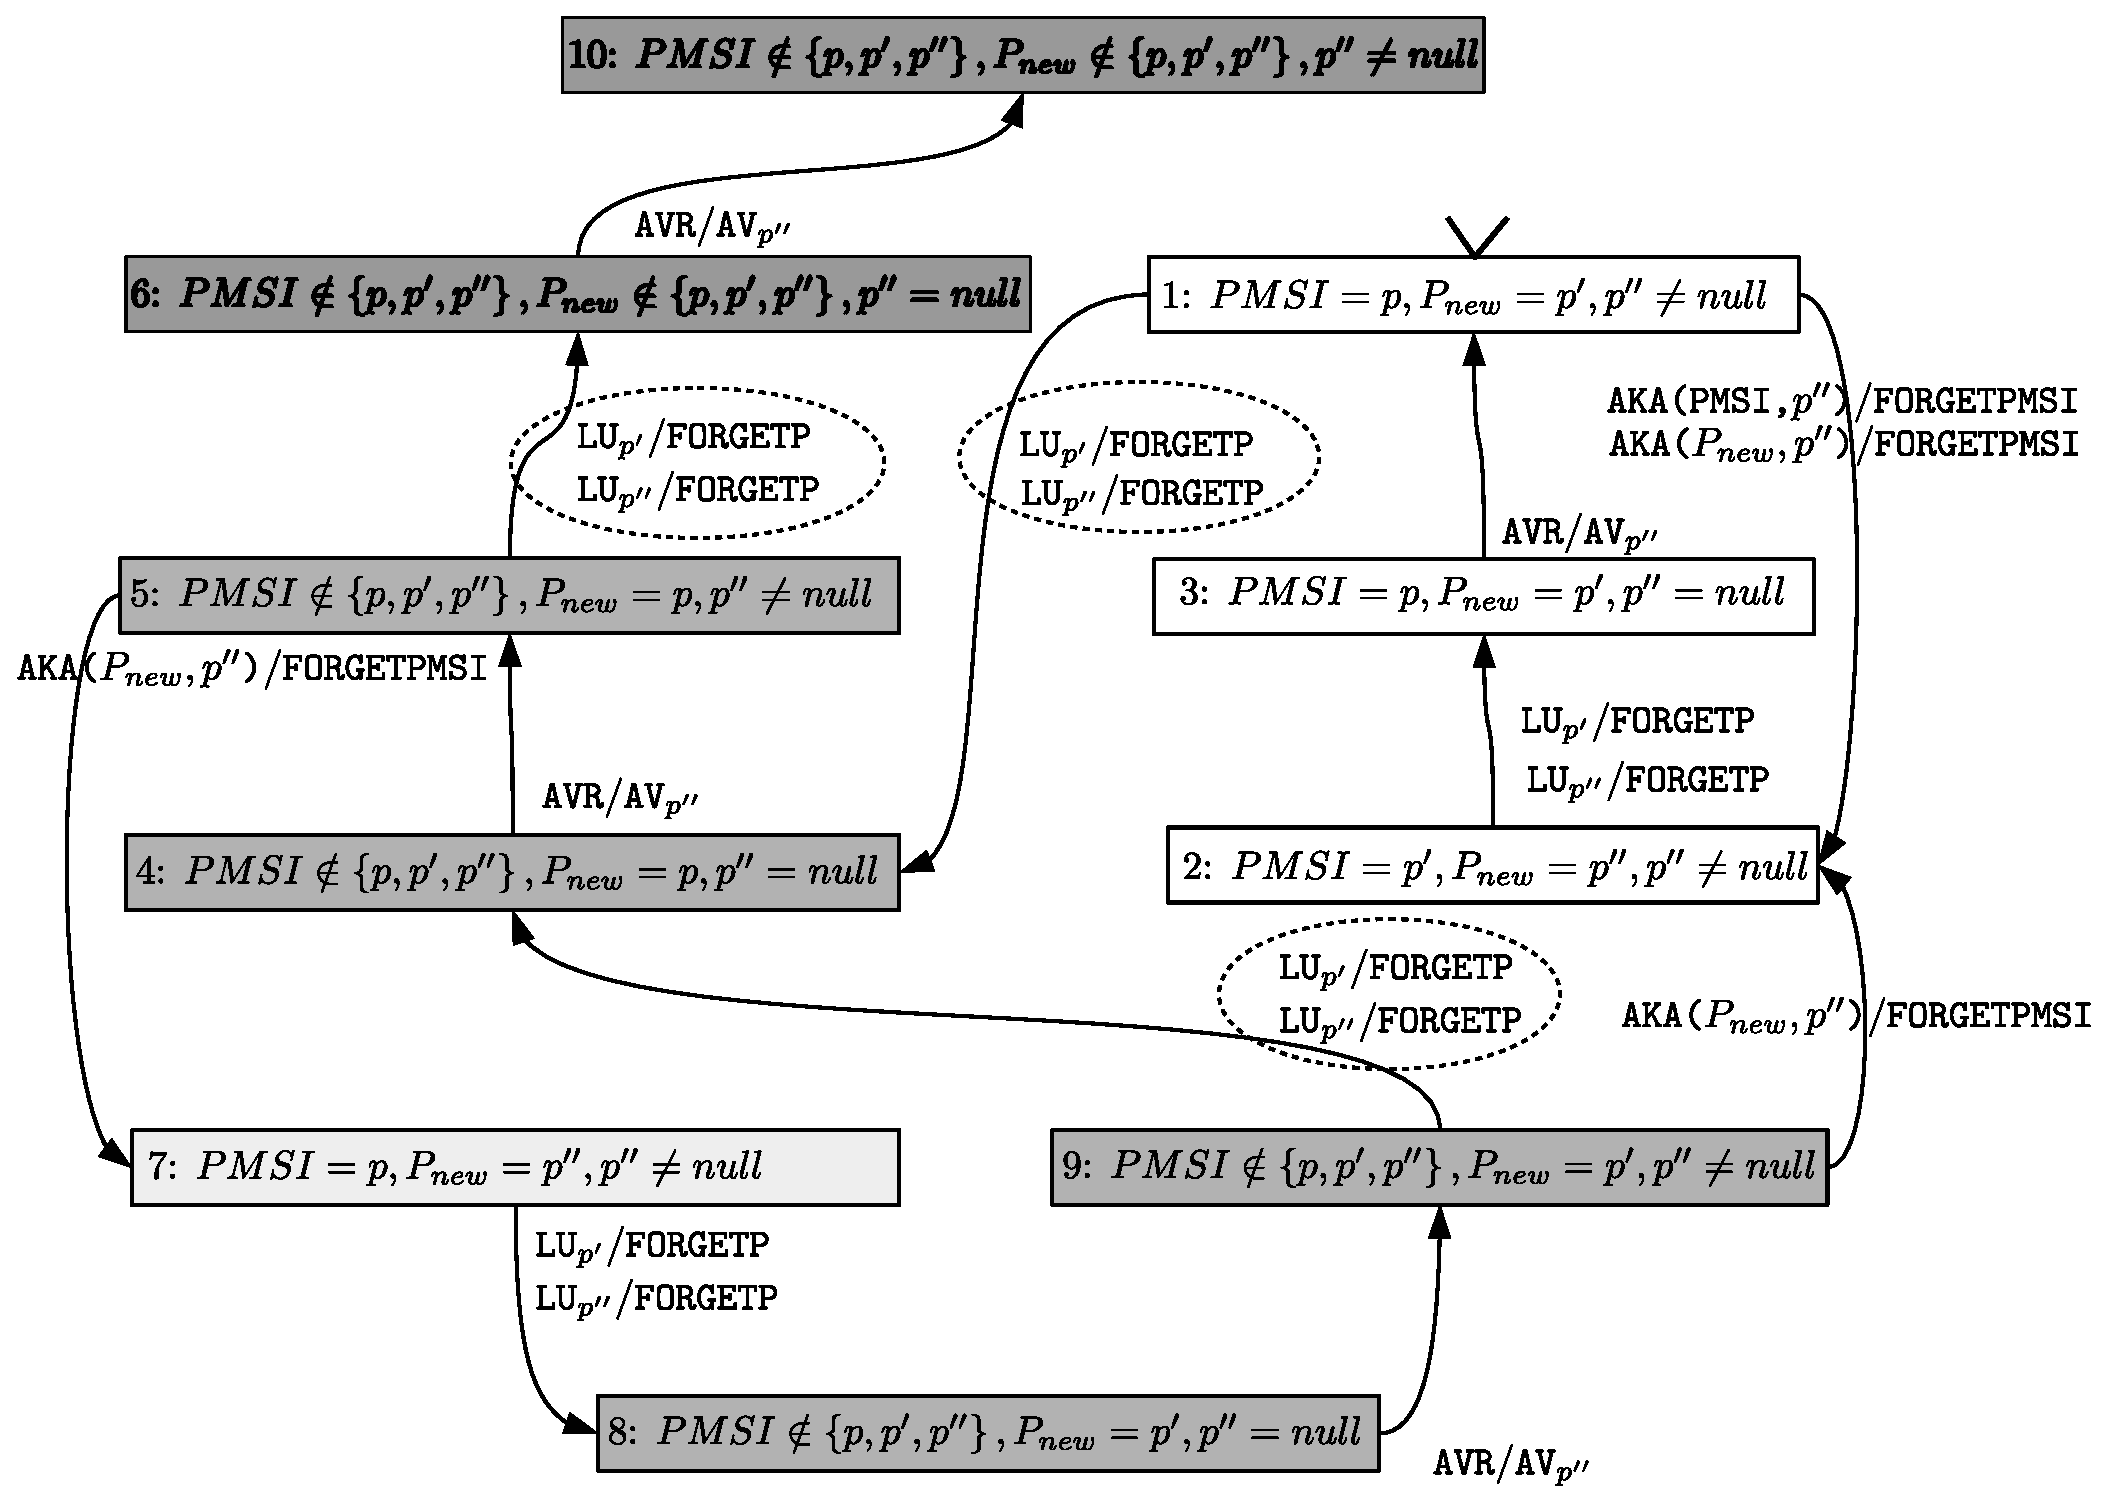
\includegraphics[scale = .35,clip = true,trim = 0cm 0cm 0cm 0cm]{solution_diagram.eps}
 \caption{Global state diagram of our solution for a user $s \in S$.}
  \label{fig:solution_diagram}
\end{figure}


\subsection{Properties of Our solution}



\textbf{Behavior of our solution in unusual but possible cases}
If an AV request is responded by the HN but the corresponding AKA is failed or not even run, then the UE keep using the pseudonyms $PMSI$ or $P_{new}$ in the upcoming AKA runs until an AKA succeeds. This can happen in global states $1$, $5$ or $9$ (Figure \ref{fig:solution_diagram}), and in this situation the global state will remain the same.

If an AKA becomes successful but the corresponding LU message is not sent to the HN then the UE will not be able to get any new pseudonym in the successive AKA runs. This can happen in global states $2$ or $7$ (Figure \ref{fig:solution_diagram}).

If because of some internal error, the $PMSI$ goes out of sync, then consequent AKA where the UE is identified by $PMSI$ will fail. However, in this case $\texttt{AKA}(P_{new},y)$ still may run where $y \notin \left\lbrace PMSI,P_{new} \right\rbrace$. Consequently the UE forgets $PMSI$ and gets back to sync. 

If because of some internal error, the $P_{new}$ goes out of sync, then consequent AKA where the UE is identified by $P_{new}$ will fail.  However, in this case $\texttt{AKA}(PMSI,y)$ still may run. Since the UE does not forget $PMSI$ after such an AKA, the UE does not update $P_{new}$ even if $y \notin \left\lbrace PMSI,P_{new} \right\rbrace$. Consequently the UE will not be able to receive any new pseudonym at all. However, a pseudonym ($PMSI$ or $P_{new}$) going out of sync because of some internal error is an extremely rare event and can be compared with the case of corrupted SIM. A user can always go to the service center of the HN and get a new SIM. Another remedy of this problem can be to maintain a list of three pseudonyms at the UE end instead of two, i.e., when $\texttt{AKA}(PMSI,y), y \notin \left\lbrace PMSI,P_{new} \right\rbrace$ happens, the UE would store $y$ as the third pseudonym even though it would not forget $PMSI$.  We have not analyzed exhaustively what happens when such a third pseudonym is introduced in the solution and can be considered as a future work.

LU messages can arrive out of order. Receiving $\texttt{LU}_{p''}$ before receiving $\texttt{LU}_{p'}$ means the UE could not get a new pseudonym when it identified itself using $p''$ and ran the consequent AKA. 

Receiving the LU messages multiple times for the same pseudonym may lead to the unsynchronized states $6$ or $10$ (Figure \ref{fig:solution_diagram}). But, as discussed later in this section, the probability of this is rather small.

%\subsection{Protection Against IMSI Catcher} 
\textbf{Protection Against IMSI Catchers} The pseudonyms are delivered to the UE encrypted by the pre-shared symmetric key $\kappa$. So, nobody except the UE can know the next pseudonym the UE will use. Hence an attacker, either active or passive, can not link a pseudonym with a previously known identity. In an ideal situation a UE uses one pseudonym in one successful AKA (notice the transitions $ \texttt{State 1} \rightarrow \texttt{State 2} \rightarrow \texttt{State 3} \rightarrow \texttt{State 1}$ in Figure \ref{fig:solution_diagram}), which is unlike the KM17 scheme. In KM17 scheme, the UE has to use one pseudonym in two successful AKAs before it can obtain a new pseudonym (see our argument in Section \ref{sec:km17scheme}). One pseudonym for one successful AKA essentially prevents an attacker to track a UE any longer than the attacker can track a UE using the TMSI or GUTI. However, the MCC and MNC part of the pseudonyms remains the same across all the pseudonyms used by a UE. Consequently if there are $k$ many users with the same MCC and MNC in the geographical area of the UE, then our solution (like BVR and KM17) provides $k$ anonymity of the user. Note that in a roaming situation $k$ may be quite small.


%\subsection{Backward Compatibility} 
\textbf{Backward Compatibility} The solution does not require any changes in the legacy SNs since no existing message format has been changed. The only changes are required in the HN and the SIM. Hence, once an HN implements the solution, any user having the upgraded SIM can enjoy the claimed identity privacy. The solution is still operable if the SIM is not updated even after the HN has implemented the solution. This is because, in our solution, the HN keep accepting the AV requests using the real IMSIs. The effect is, the UE will not be able to extract the new pseudonyms from the $RAND$. Otherwise everything else remains same and operable. 

Our solution builds on top of UMTS/LTE AKA without introducing any new messages or changes in any existing messages. Hence solution will provide the claimed privacy in the presence of SNs from UMTS and LTE networks too. 


A legacy SN may fetch multiple AVs from the HN for a single pseudonym $x$. Since $\texttt{AKA($x,y$)}$ where $x= PMSI$ does not trigger any pseudonym update, let us consider the cases where $x=P_{new}$, i.e.,
$\texttt{AKA($P_{new},y$)}$. In such cases, if $y \notin  \left\lbrace PMSI,P_{new} \right\rbrace$ then the UE forgets $PMSI$ and the $P_{new}$ becomes the new $PMSI$. Consequently if the SN uses the pre-fetched AVs thereafter, it would be the $\texttt{AKA($PMSI,y$)}$ cases -- which has no impact on the pseudonym states of a user. Hence, our solution works smoothly even when an SN uses pre-fetched AVs for a pseudonym $x$ unless some other user in the same SN is assigned with pseudonym $x$. Let us assume a user $s_1$ receives a new pseudonym $x$ from the HN and sets $P_{new} \leftarrow x$. Then user $s_1$ uses $P_{new}=x$ in an SN where the SN already has a pre-fetched AV for the pseudonym $x$ associated with user $s_2$ (forgotten by both HN and UE of $s_2$). In this case, user $s_1$'s AKA will fail. But it is also very unlikely to happen. If it happens, the user $s_1$ can still run $\texttt{AKA($PMSI,y$)}$. However, such AKAs will not enable the UE to receive a new pseudonym. One remedy of this problem can be that the UE may trigger an $SQN$ resynchronization process if an AKA fails after identifying using $P_{new}$. By triggering such an $SQN$ resynchronization process, the UE may force the SN to get a fresh AV from the HN.

%\subsection{Protection Against the DDos Attack} 
\textbf{Protection Against the DDos Attack:} The DDoS attack is mounted by a botnet of mobile devices. The objective of the attack is to bring as many mobile users as possible to bring to State $6$ of Figure \ref{fig:solution_diagram}. However, any path in the state diagram (Figure \ref{fig:solution_diagram}) that leads to State $6$ involves at least one LU message. An SN will send an LU message for a pseudonym only if the corresponding AKA was successful. A mobile bot can not participate in a successful AKA with an SN using an arbitrary pseudonym. Hence, the attack does not work without an SN helping the botnet to do so.


%\subsection{Protection Against a Malicious or Buggy SN} \label{sec:attack_by_malicious_buggy_SN}
\textbf{Protection Against a Malicious or Faulty SN:} In principle, a malicious SN can still attack the HN by sending a fake LU message for pseudonyms $p',p''$ that are associated with legitimate users. The target of the attacker would be to send a user to state $6$ of the state diagram in Figure \ref{fig:solution_diagram}. We will show that the probability of success for such an attack is very low before the attack is detected and stopped. Besides an SN is in a roaming contract (it is a business contract) with an HN. The minimal harm the SN can cause to the HN before the attack is detected and stopped is not worth of risking the renewal of the contract.

Notice the paths that lead to state $6$ in Figure \ref{fig:solution_diagram}. All such paths go via state $4$. Let us assume that all the users of the HN are currently in State $1$ or $9$. This is a safe assumption because otherwise the attack would be even less likely to succeed. The malicious SN has to send fake $\texttt{LU}_{p'}$ or $\texttt{LU}_{p''}$ to reach State $4$. This implies that the malicious SN needs to know either $p'$ or $p''$ of a legitimate user $s$. The attack can be analyzed for two different situations. In one where the target users are currently not visiting the malicious SN. In other the target users are visiting the malicious SN.

%\subsubsection{Target Users are not Visiting the Malicious SN} 
\textit{Target Users are not Visiting the Malicious SN:} The malicious SN can try to mount a DoS attack against an HN targeting the users who are not even visiting the SN. In that case, the malicious SN guesses $q=p''$ and send a LU for $q$ to the SN. This brings the user to State $4$. Then the malicious SN sends an AV request to the HN using $q$ . This brings the user to State $5$. Then the SN sends another LU for $q$. This time the user goes to State $6$. So the attack is basically a sequence of LU message, AV request and another LU message using the same guessed pseudonym $q$. Let us consider that the SN starts from $0$ and choose incrementally all the possible pseudonyms across the whole space and send the three messages to the HN using the chosen pseudonyms $q$. In that way after sending $m$ triplets of messages to the HN, the expected number of affected users would be $\frac{nm}{\mathcal{M}}$. %Figure \ref{fig:expected_success_rate_attack_all_by_sn} shows the expected number of affected subscribers as $m$ grows where $n$ is the total number users of the HN.

%\subsubsection{Target Users are Visiting the Malicious SN} 
\textit{Target Users are Visiting the Malicious SN:} If the target users are currently visiting the malicious SN, it is easy to know the users' $p'$ because the UE gives it to the SN. The malicious SN makes IMSI inquiries to all the UEs and hope that most of the UEs will respond with $P_{new} = p'$. Then the malicious SN sends LU messages for all the pseudonyms received as the respond of the IMSI inquiries. This brings many of the users to State $4$.  Once at State $4$, the malicious SN can send an AV request to the HN using $p'$ which will take the user from State $4$ to State $5$. However, once at State $5$, neither the UE nor the malicious SN knows $p',p''$. So, to reach to State $6$, the malicious SN has to guess one of $p',p''$ exhaustively. Suppose it starts from $0$ and incrementally choose all the possible pseudonyms across the pseudonym space and send LU messages for the chosen pseudonyms to the HN. By doing so, after sending $m$ LU messages to the HN, the expected number of users that will reach State $6$ is at most $\frac{2rm}{\mathcal{M}}$, where $r$ is the number of users currently visiting the malicious SN. %Figure \ref{fig:expected_success_rate_attack_by_sn_insider} shows the expected number of affected subscribers as $m$ grows for different values of $r$.

To summarize, a malicious SN can attack the users of an HN by sending to an HN LU messages with randomly chosen pseudonyms. But the HN can detect and counter the above attack: In order to desynchronize at least one user of the HN on the average, the malicious SN has to send more than $m \geq \mathcal{M}/n$  LU messages with randomly chosen pseudonyms. (Remember that $n$ is the total number of users having the same MCC, MNC in the HN, and $\mathcal{M}$ is the size of MSIN space, which we assume is $10^{10}$.) For example, if $n=10^8$, then the number of those messages should be at least $10^{10}/10^{8}$, i.e.~100; and if $n=10^6$, then the number of those messages should be at least ~$10^4.$
 
But the malicious SN has a large, $1 - n/\mathcal{M}$ chance to guess the pseudonym wrongly in any given LU message; resulting in LU for a pseudonym not belonging to any user of the HN. Even a few such messages should make the HN realize that there is a de-synchronization attack. The HN could then apply countermeasures. For example, in the short term, HN could temporarily suspend processing any LU messages coming from the SN. This will make the UEs who are visiting the malicious SN more easy to track for the duration of suspension (because they will have to use the same pseudonym), but on the other hand, it will prevent de-synchronization of their pseudonyms. And in the long term, the HN may choose not to renew the roaming agreement with the operator of the SN.


%\begin{figure}[]
%  \centering
%  \begin{minipage}[b]{0.49\textwidth}
%    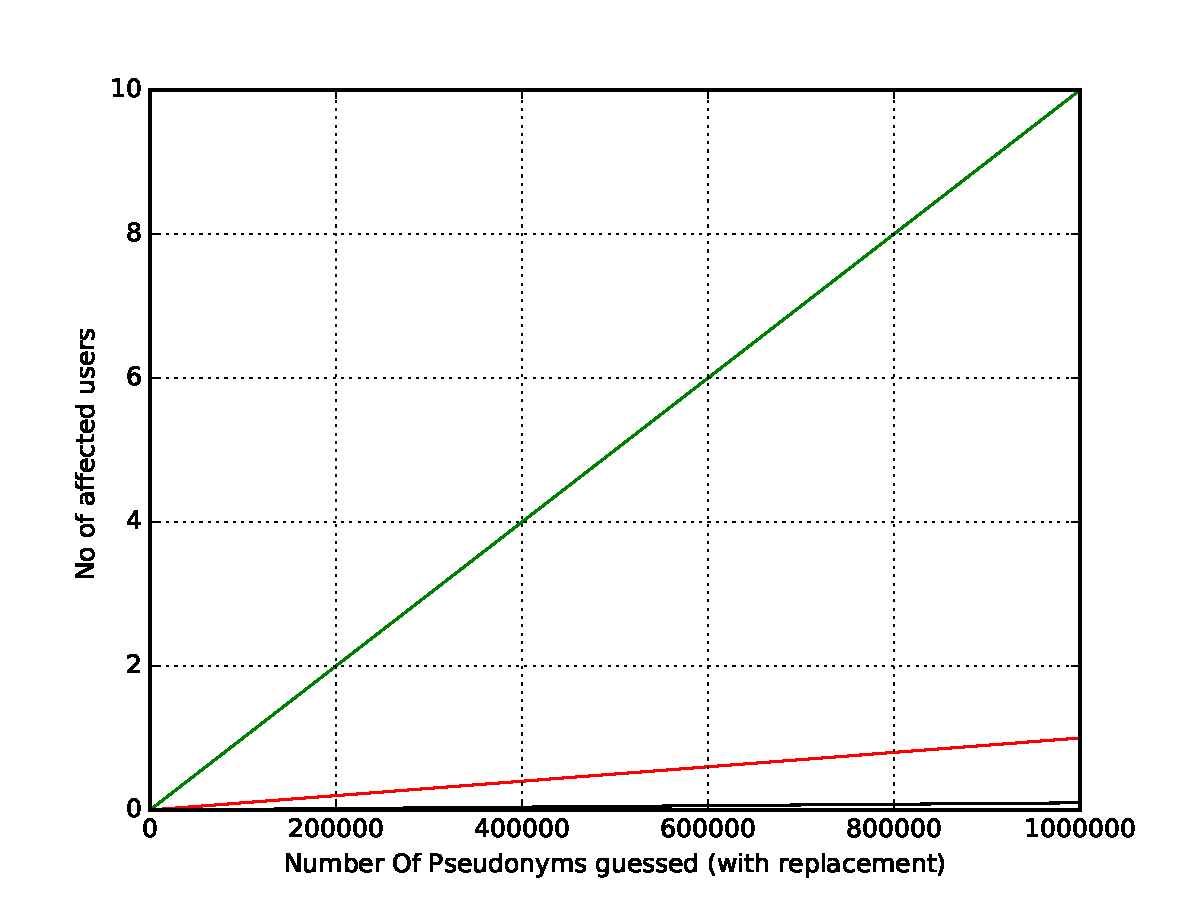
\includegraphics[width=\textwidth]{expected_success_rate_attack_by_sn_insider.pdf}
%   \caption{Expected number of affected subscriber in the attack by SN. The attack is targeted to the subscribers who are visiting the SN.}
%\label{fig:expected_success_rate_attack_by_sn_insider}
%  \end{minipage}
%  \hfill
%  \begin{minipage}[b]{0.49\textwidth}
%    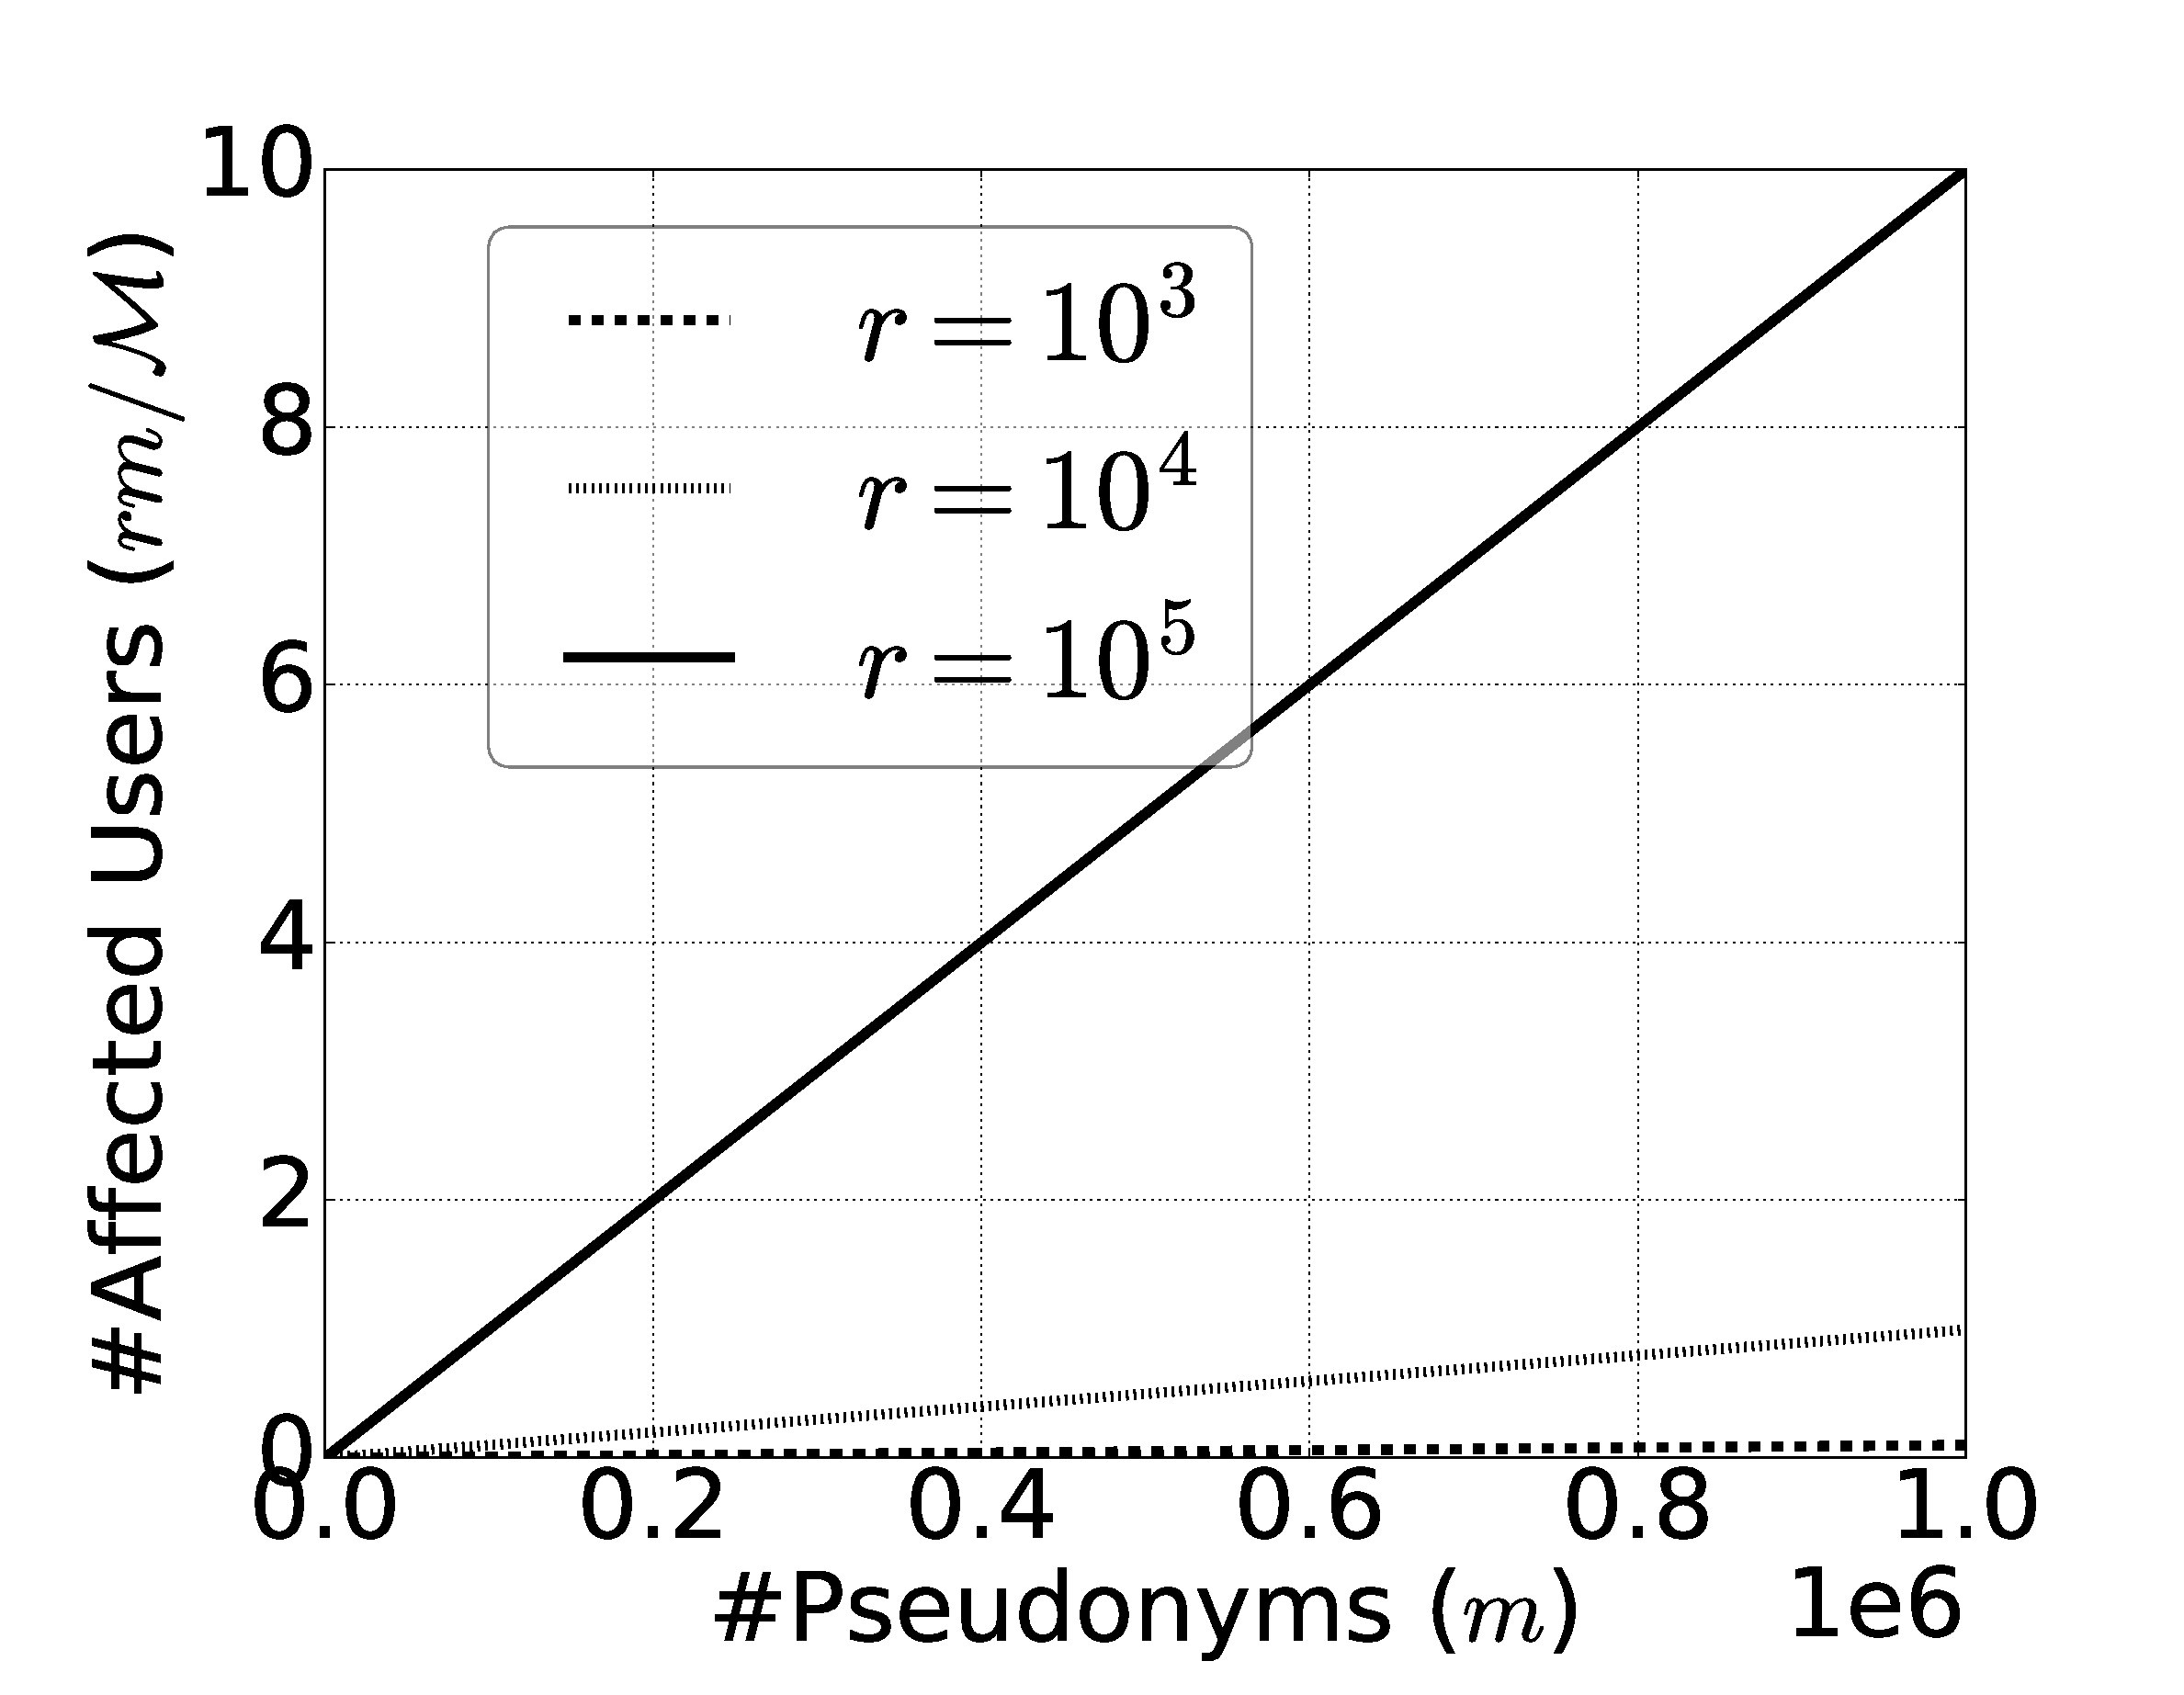
\includegraphics[width=\textwidth]{sn_attack_all.pdf}
%    \caption{Expected number of affected subscriber in the attack by SN. The attack is targeted to all subscribers of the HN.}
%  \label{fig:expected_success_rate_attack_all_by_sn}
%  \end{minipage}
%\end{figure}



%\subsection{Protection Against Replay Attack by SN} \label{sec:replay_attack_sn}
\textbf{Protection Against Replay Attack by an SN:} A malicious SN may store an AV that it received from the HN with an intention to use later in an AKA with a UE. If the SN could do so, then a UE can be tricked to accept an old pseudonym which is already forgotten at HN. However, an SN can not do that. The pseudonyms are send to the UEs encrypted. No one including the SN knows the pseudonym before it is used by a UE. Consequently the malicious SN would know a valid AV for a UE identified by the pseudonym $p$ only if the AV was obtained from the HN by making an AV request using the same pseudonym $p$. The next pseudonym embedded in such an AV can not be forgotten by either the UE or the HN. Hence a malicious SN can not make a replay attack to a targeted UE. However, the malicious SN can use an stored AV to run AKA with all the UE who are visiting the SN. In that case one user may get affected if the $SQN$ in the AV is still fresh. This may imply that the valid range of $SQN$ has to be small when a UE is in roaming.



%\subsection{Charging and Lawful Interception}
\textbf{Charging and LI:} The HN has to keep track of the pseudonyms used by a particular user over time. This is needed, first, in order to bill the (right) user. Since the bills are typically settled once per month, the pseudonym usage records have to be retained for at least one month. Second, this is required for lawful surveillance of telecom traffic. The retention period of the records may be different in different countries, but in general, it will be longer than one month. For example, the European Union's Data Retention Directive \cite{dataretention} required to store call related data for a period of time between six and 24 months. The need of law enforcement agencies to know in real time the true identity of the mobile user can be met by the HN sending that identity to the SN during the connection establishment. But the handling of this identity would be a new feature in the legacy SN. When deploying pseudonym-based enhancements to user identity privacy, some parts in the SN may have to be upgraded to meet law enforcement needs.





%As the pseudonyms are frequently changing and one pseudonym may be used by many users over the time, the blling and charging system of HN needs to keep track of the time a pseudonym is used by a particular user. This implies that the HN needs to remember the history of the use of pseudonyms for a while so that two mobile operators who have a roaming contract can settle their bills. Usually the roaming partners settle their bills once in a month. This implies that the pseudonym history has to be retained for at least a month. On the other hand, for lawful interception (LI) purpose the history might needed to be remembered for quite a longer time, depends on the law of the land. The retention of the pseudonym history might become an overhead for the HN. However, it is just a mapping from the pseudoynms to the pairs $(IMSI,\text{date})$ and should not be a deal breaker for using pseudonyms.

%\subsection{Performance Overhead}
\textbf{Performance Overhead:} A random choice of next pseudonym, the encryption of the pseudonym is the additional overhead in generating an AV. This should not be too much for an HN. The retention of the history of pseudonyms is also an additional overhead but does not impact the generation of AVs. In the SIM it adds one extra key and one decryption using the key. The SNs would see more users registering in the network because when a UE forgets a pseudonym, it does not inform the SN. However, the legacy SNs are familiar with cases where a UE suddenly powers off, and a UE forgetting an old pseudonym would just be treated as the UE has powered off.

%\subsection{Parameter Choice}
\textbf{Parameter Choice:} The encryption used in encrypting the pseudonyms will not have forward secrecy since the same key $\kappa$ is used all the time for encrypting pseudonyms. We have used $34$ bits (as the BVR scheme) for next pseudonym in the $RAND$ instead of $4$ bits per digit. This makes sense because the UE can convert it back into the required format. Besides, using less amount of bits for pseudonym encoding leaves room for the length of the $salt$, denoted by $l$ be longer. If the cipher used for encrypting $u=\left(p'',SQN,salt\right)$ has block length $128$, then embedding the same $p''$ in the successive $RAND$s can be randomized by the $48$ bit long $SQN$ and a $46$ bit long $salt$. As the same $p''$ might be sent over successively many $RAND$s, the cipher used for encrypting $u$ to generate $RAND$ should be immune against related plaintext attack \cite{CCS15}. AES is used in UMTS and LTE network for the implementation of authentication function and immune against related plaintext attack. So it would be enough to use AES for encrypting pseudonym also \cite{CCS15}. 


\section{Conclusion} \label{sec:conclusion}
The need to maintain synchronized state between the UE and the home networks is one of the key issues in the design and implementation of pseudonym-based enhancements of user identity privacy in mobile networks. In this paper we have proposed  a relatively simple design for a layer of pseudonyms between UE and home network that can withstand de-synchronization attacks. This gives hope that pseudonym-based solutions can be applied in commercial cellular networks. Topics for future work include formal verification of our scheme, and its implementation and testing using real UEs and mobile network elements.


\subsubsection{Acknowledgement.}
\label{sec:acknowledgement}
We thank Markku Antikainen for the useful discussion to characterize the DDoS attack and his help to optimize the code of the simulation of the DDoS attack.


\bibliographystyle{splncs}
\bibliography{ref}{}

%\begin{thebibliography}{5}



%\end{thebibliography}


\begin{subappendices}
\renewcommand{\thesection}{\Alph{section}}%
% or try \arabic{section}

\section{} \label{appendix:A}
Let us consider that there are $\mathcal{M}$ number of bins, each labeled by a pseudonym or IMSI. Choosing $m$ random pseudonym with replacement and sending them in an attach request can be compared with the classic experiment of throwing $m$ balls to $\mathcal{M}$ bins. The number of affected users by sending $m$ number of attach requests is same as the number of bins that get two or more balls after throwing $m$ balls to $\mathcal{M}$ bins. The probability that a particular bin gets no balls is $\left(1-\frac{1}{\mathcal{M}}\right)^m$. The probability that this bin get exactly one ball is $\binom{m}{1}\frac{1}{\mathcal{M}}\left(1-\frac{1}{\mathcal{M}}\right)^m$. Consequently, the probability that the bin will get two or more balls is:
\begin{eqnarray*}
 1 - \left(1-\frac{1}{\mathcal{M}}\right)^m - \binom{m}{1}\frac{1}{\mathcal{M}}\left(1-\frac{1}{\mathcal{M}}\right)^m
\end{eqnarray*}
If $n$ is the number of users in the HN, then by linearity of expectation, the expected number of affected user would be:
\begin{eqnarray*}
 n\left(1 - \left(1-\frac{1}{\mathcal{M}}\right)^m - m\frac{1}{\mathcal{M}}\left(1-\frac{1}{\mathcal{M}}\right)^m\right)
\end{eqnarray*}
Consequently the expected portion of affected user would be:
\begin{eqnarray*}
 E[u_a] = 1 - \left(1-\frac{1}{\mathcal{M}}\right)^m - m\frac{1}{\mathcal{M}}\left(1-\frac{1}{\mathcal{M}}\right)^m
\end{eqnarray*}


\section{} \label{appendix:B}
In the without replacement attack, the attacker sends all the pseudonyms incrementally starting from $0$ across the whole MSIN space. Let us consider that the pseudonym $x$ is the first attack on a user's $p'$. Once the user's $p'$ is attacked, HN updates $p \leftarrow p'$ and choose a new unused $p'$ randomly. If the attacker sends total $m$ number of pseudonyms to the HN, then the probability that the user's new $p'$ will once again be attacked is: $\frac{m-x}{\mathcal{M}}$. If $n$ is the total number of subscribers in the HN and $m \leq \mathcal{M}$ (first round) then expected number of subscribers affected after sending $m$ pseudonyms is:
\begin{eqnarray*}
 \frac{n}{\mathcal{M}}\int_{0}^{m}\frac{m-x}{\mathcal{M}}dx &=& \frac{n}{\mathcal{M}^2}\int_{0}^{m}\left(m-x\right)dx\\
 &=& \frac{nm}{\mathcal{M}^2}\int_{0}^{m}dx - \frac{n}{\mathcal{M}^2}\int_{0}^{m}xdx\\
 &=& \frac{nm^2}{\mathcal{M}^2} - \frac{nm^2}{2\mathcal{M}^2}\\
  &=& \frac{nm^2}{2\mathcal{M}^2}
\end{eqnarray*}
Consequently, the expected portion of affected users would be $\frac{m^2}{2\mathcal{M}^2}$ where $m \leq \mathcal{M}$.

\paragraph{} Let us now consider the case where $\mathcal{M} < m \leq 2\mathcal{M}$ (second round). The attacker again sends all the pseudonyms incrementally starting from $0$. Choosing a pseudonym $x$ will affect a user (who has not yet been affected) only if $x$ is the pseudonym of a user who was attacked only once in the first round. The probability of that event is: $1 - \frac{x}{\mathcal{M}}$. So, after sending $m = \mathcal{M} + m'$ number of pseudonyms, the expected number of affected user would be:
\begin{eqnarray*}
 & & \frac{n\mathcal{M}^2}{2\mathcal{M}^2} + \frac{n}{\mathcal{M}} \int_{0}^{m'}\left(1 - \frac{x}{\mathcal{M}} \right)dx \\
 &=&  \frac{n}{2} + \frac{n}{\mathcal{M}} \int_{0}^{m'}\left(1 - \frac{x}{\mathcal{M}} \right)dx \\
 &=& \frac{n}{2} + \frac{n}{\mathcal{M}^2} \int_{0}^{m'}\left(\mathcal{M} - x \right)dx \\
 &=& \frac{n}{2} + \frac{n}{\mathcal{M}^2} \int_{0}^{m'} \mathcal{M} dx  - \frac{n}{\mathcal{M}^2} \int_{0}^{m'} x dx \\
  &=& \frac{n}{2} + \frac{nm'}{\mathcal{M}} - \frac{n}{\mathcal{M}^2} \frac{m'^2}{2} \\
  &=& \frac{n}{2} + \frac{n\left( m - \mathcal{M} \right)}{\mathcal{M}} - \frac{n}{\mathcal{M}^2} \frac{\left( m - \mathcal{M} \right)^2}{2} \text{(since }  m = \mathcal{M} + m' \text{)}\\
 % &=& \frac{n}{\mathcal{M}} \left( \frac{\mathcal{M}}{2} + \left( m - \mathcal{M} \right) - \frac{1}{\mathcal{M}} \frac{\left( m^2 - 2m\mathcal{M} + \mathcal{M}^2 \right)}{2} \right) \\
 % &=& \frac{n}{\mathcal{M}} \left( \frac{\mathcal{M}^2 + 2 m\mathcal{M} - 2 \mathcal{M}^2 - m^2 + 2m\mathcal{M} - \mathcal{M}^2}{2\mathcal{M}} \right) \\
 % &=& \frac{n}{\mathcal{M}} \left( \frac{4m\mathcal{M} - 2\mathcal{M}^2 -m^2}{2\mathcal{M}} \right) \\
    &=& \frac{n}{\mathcal{M}} \left( 2m - \mathcal{M} - \frac{m^2}{2\mathcal{M}} \right) \\
\end{eqnarray*}

Consequently, the expected portion of affected users would be $\frac{1}{\mathcal{M}} \left( 2m - \mathcal{M} - \frac{m^2}{2\mathcal{M}} \right)$ where $\mathcal{M} < m \leq 2\mathcal{M}$.

\paragraph{} Even though $x$ in the above derivation is a discrete variable, we have used integration. So, the result we have found here is an approximation. We expect it to be a good approximation.


\end{subappendices}


\end{document}
